\documentclass[11pt]{article}
\usepackage[a4paper,margin=2.35cm]{geometry}
\usepackage{amsmath,amssymb,amsthm,mathtools,bm}
\usepackage{booktabs,longtable,tabularx,array}
\usepackage{graphicx}
\usepackage{xcolor}
\usepackage{microtype}
\usepackage{hyperref}
\usepackage[numbers,sort&compress]{natbib}
\usepackage{enumitem}
\usepackage{placeins}

\setlength{\emergencystretch}{2em}
\hypersetup{
  colorlinks=true,
  linkcolor=blue!45!black,
  citecolor=blue!45!black,
  urlcolor=blue!45!black
}

\newtheorem{definition}{Definition}
\newtheorem{theorem}{Theorem}
\newtheorem{proposition}{Proposition}
\newtheorem{corollary}{Corollary}
\newtheorem{remark}{Remark}
\newcolumntype{L}[1]{>{\raggedright\arraybackslash}p{#1}}

\newcommand{\At}{\mathfrak A}
\newcommand{\Temp}{\operatorname{Temp}}
\newcommand{\Desc}{\operatorname{Desc}}
\newcommand{\Stab}{\operatorname{Stab}}
\newcommand{\im}{\operatorname{im}}
\newcommand{\rank}{\operatorname{rank}}
\newcommand{\Tr}{\operatorname{Tr}}
\newcommand{\Id}{\mathrm I}

\title{\textbf{Temporalization of an Atemporal Parent}\\
\large Morphogenesis, Actuality, Observer Time, and Empirical Identifiability in Tau Core}
\author{Jozsef Olcsak\\\small Independent researcher}
\date{Preparation manuscript --- Last revised: 3 September 2026}

\begin{document}
\maketitle

\begin{abstract}
The Tau Core foundation sequence separates an atemporal morphological parent,
physical source realization, observer-relative temporal descent, quantum
records and four-dimensional terminal physics.  A long subsequent
morphogenesis program developed these layers in detail but left its net
result distributed across many conditional constructions, no-go theorems and
negative data preflights.  This paper gives a nonredundant synthesis.  It
imports, without re-proving, the component results of Foundation Papers
I--VII and states one typed composition theorem.

The conservative architecture is not a competition between an atemporal and
a temporal ontology.  Temporalizable carriers form a subclass of atemporal
parent bodies, while a temporal completion is a fibered enhancement carrying
a source-owned order structure.  On a finite retained relation complex, a
prescribed scalar proto-time exists exactly when the occurrence cochain has
zero signed period on every cycle after physical-null descent.  In the
declared enriched actuality completion, a complete quotient-basic occurrence
action selects the exact cochain
\(\omega_{\rm occ}=-d\mathcal A_{\rm occ}\), and the EOCC response
\(X_{\rm EOCC}=-\Gamma^{-1}d\mathcal A_{\rm occ}\) gives
\(\omega_{\rm occ}(X_{\rm EOCC})>0\) away from equilibrium.  This proves
monotone action descent, progressive stabilization and a finite parent-action
formation budget inside that completion.  It does not derive EOCC from the
static minimal theory or prove that Nature occupies the enriched model.

Observer time is a later body-conditioned, source- and observer-dependent
readout.  Stable quantizer cells, record instruments and calibration are
required before proto-order becomes an operational clock.  A frozen past is
therefore persistence of compatible prefix restrictions and stable records,
not a parent memory store.  Neither EOCC order nor record persistence alone
selects an entropy arrow.  Entropy growth follows conditionally from a
source-owned non-erasing visible refinement with one consistent ensemble;
thermodynamic promotion additionally requires a physical macroterminal,
conserved constraints and an equilibrium measure.  Common ownership of the
actuality and readout packet does not fix the macroterminal sign.  A minimal
free-action completion proves local thermodynamic growth only after a
positive temperature-like scale and conservation law are supplied.  More
sharply, a symmetric configuration Laplacian has an exact logarithmic-mean
EOCC representation and free-action decomposition.  This thermal production
need not equal the entropy of a refined front readout.  Every finite source-frozen acyclic process in the
declared intervention class has an operationally identical atemporal
simultaneous factorization; unrestricted finite internal data cannot identify
literal ontic traversal.  A lawful test must instead freeze a bounded
atemporal comparator and detect a source-owned nonfactorizing rank, capacity
or record effect.  Existing public-data preflights do not yet supply such a
signal.  Finally, a conditional four-dimensional exchange current can carry
the finite formation budget, but its units, receiver equation of state,
localization and dark-sector split are not selected.  The current status is a
mathematically specified conditional temporal working completion with exact
internal theorems and exact observational ceilings, not an empirically
supported theory of parent time. A generalized observer-access theorem also
allows the terminal decomposition of one accessible parent quotient to vary
between observers. This simultaneous factorization does not temporalize the
Parent and does not make distinct terminal laws interchangeable.
\end{abstract}

\begin{center}
\fbox{\begin{minipage}{0.92\linewidth}\small
\textbf{Nonredundancy and ownership.}
Foundation Paper I owns the atemporal parent/readout architecture; Paper II
the typed source-signature constraints; Paper III record transport; Paper IV
the parent-law realization and actuality boundary; Paper V temporal descent,
exact finite temporalizability and the interventional simulation no-go; Paper
VI quantizer, complete-record and history-refinement results; Paper VII the
conditional 4D terminal boundary.  This paper does not reproduce those
derivations.  It owns their typed composition, the consolidated current-status
ledger and the resulting proof/falsification ladder.
\end{minipage}}
\end{center}

\begin{center}
\fbox{\begin{minipage}{0.92\linewidth}\small
\textbf{Claim boundary.}
Nothing below proves that old-bare Tau entails an actuality law, that Nature
selects the enriched temporal completion, that an absolute parent clock
exists, or that observer time equals proto-time.  No SI clock or energy unit,
dark component, cosmological anomaly, quantum anomaly, or Tau Core signal is
derived from the temporal construction.  Conditional mathematical closure is
kept separate from physical source selection and empirical validation.
\end{minipage}}
\end{center}

\tableofcontents
\clearpage

\section{Question, method and relation to the foundation sequence}

The research question is deliberately narrower than ``does time exist in the
Parent?''  It is
\begin{quote}
Under which source-owned conditions can an atemporal parent morphology carry
an integrable, physically actual temporalization whose observer descent has
operational consequences, and which observations could distinguish that
completion from a controlled atemporal comparator?
\end{quote}

The foundation sequence already fixes the direction
\begin{equation}
 B_\tau^{\rm phys}+s_U
 \longrightarrow M_\tau
 \longrightarrow \mathcal C_{OS}(M_\tau)
 \longrightarrow \mathcal R_{OS}
 \longrightarrow Y_{OS}^{(a)},
 \label{eq:foundation-spine}
\end{equation}
where \(s_U\) is one universal morphology seed, \(M_\tau\) is the stabilized
morphological response configuration (short name: morphological body),
\(\mathcal C_{OS}\) is the body-conditioned full
observer--source channel, \(\mathcal R_{OS}\) is a shared resolved descriptor
and \(Y_{OS}^{(a)}\) denotes typed terminal readouts.  The body is not
constructed backward from a clock, quantum outcome, residual or cosmological
fit \citep{TauFoundationI2026,TauFoundationII2026,TauFoundationIII2026}.

Paper IV isolates the physical source-realization question and the additional
actuality content required by a temporal completion
\citep{TauFoundationIV2026}.  Paper V derives temporal descent and observer
clocks from an already available body packet, not the body from time
\citep{TauFoundationV2026}.  Papers VI and VII then constrain record and 4D
terminal interpretations \citep{TauFoundationVI2026,TauFoundationVII2026}.
This manuscript composes those arrows once.  It does not make each terminal
paper repeat the parent architecture.

The method has four rules.
\begin{enumerate}[label=(M\arabic*)]
\item Every imported result retains its canonical owner and premise set.
\item A current net verdict replaces superseded intermediate gates; negative
      paths remain provenance, not additional positive claims.
\item Every positive completion is accompanied by an identical-reduct or
      deletion control showing which additional premise carries the result.
\item Internal mathematical closure, Nature-level source selection and
      empirical discrimination are reported at different levels.
\end{enumerate}

Figure~\ref{fig:dependency} summarizes the ownership map.  The full compact
ledger is included in the reproducibility package.

\begin{figure}[t]
\centering
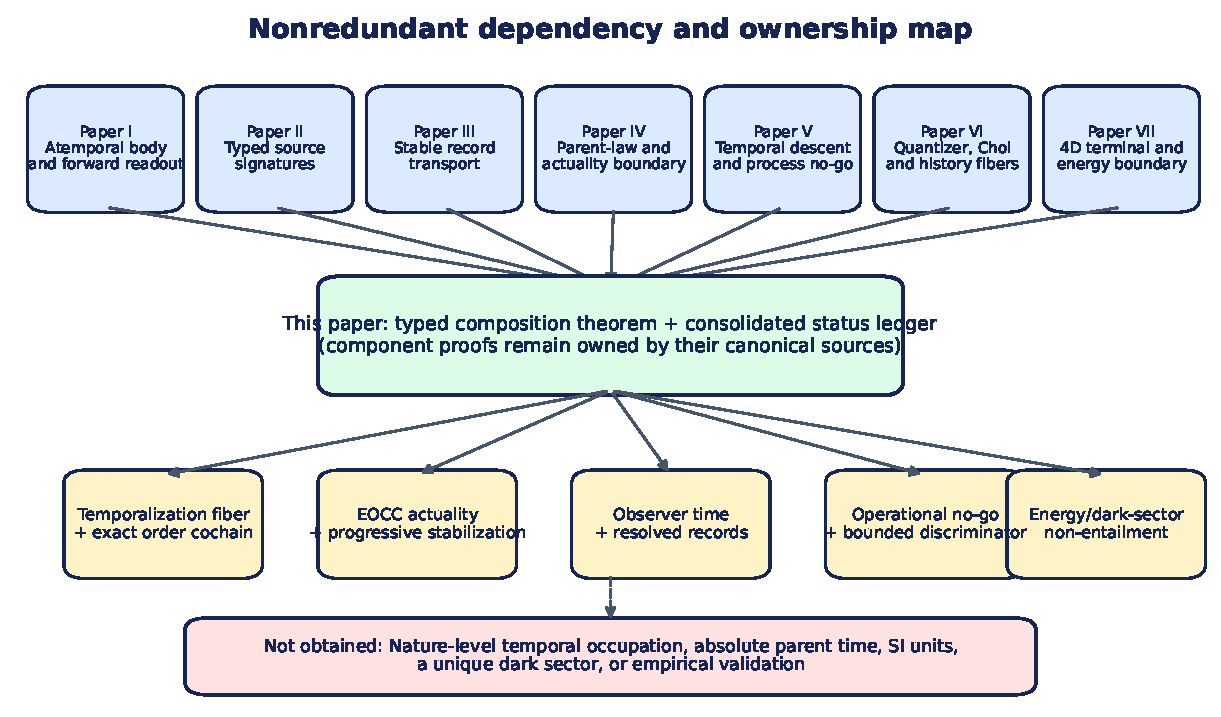
\includegraphics[width=\linewidth]{figures/fig_dependency_ownership_map.pdf}
\caption{Nonredundant dependency map.  Blue boxes are inherited foundation
results, the green box is the composition owned here, yellow boxes are
conditional consequences, and the red box records conclusions that do not
follow.  Arrows denote logical dependence, not parent-time evolution.}
\label{fig:dependency}
\end{figure}

\section{Inherited-results ledger}

Table~\ref{tab:ownership} is the paper-facing dependency ledger.  ``Exact''
always means exact on the declared finite or regular domain, not physical
selection by Nature.

\small
\begin{longtable}{@{}L{0.12\linewidth}L{0.21\linewidth}L{0.25\linewidth}L{0.25\linewidth}@{}}
\caption{Inherited results, owners and use in this synthesis.}\label{tab:ownership}\\
\toprule
Owner & Imported object & Status retained here & Use; not repeated here \\
\midrule
\endfirsthead
\toprule
Owner & Imported object & Status retained here & Use; not repeated here \\
\midrule
\endhead
Paper I & Atemporal body and forward parent-to-readout direction &
Architecture plus conditional MVP & Fixes Eq.~\eqref{eq:foundation-spine} \\
Paper II & Typed source signatures and joint incidence &
Finite exact/conditional representation results; one joint
$\mathfrak J_*=(\Pi_*,\varphi_*)$ fixes mixed ideal, separator multiplicity,
relative gluing and faithful block occupation & Prevents untyped source
identification and independent retuning of those four descendants \\
Paper III & Complete record edges and recovery-correctable transport &
Exact and conditional record results & Supplies stable record transport
without parent history storage \\
Paper IV & Parent-law realization and EOCC boundary &
Conditional completion plus non-entailment & Separates stationary body
realization from physical actuality \\
Paper V & Temporalization fiber, order, clocks and finite process no-go &
Exact finite theorems under declared assumptions & Supplies the temporal
descent layer \\
Paper VI & Observer quantization, complete record jets and no-retro refinement &
Conditional quantum/readout theorems & Supplies the operational record layer \\
Paper VII & Gravity, matter and gauge assembly &
Conditional terminal recovery only & Blocks direct identification of actuality
with 4D stress-energy \\
TMB 379--391 & Seed key, body realization and internal-observer ontology &
Typed ontology decision & Fixes the meaning of seed, body and observer \\
TMB 402--424 & Lossy relay, stabilization, EOCC working completion and budget &
Conditional theorem family with exact controls & Supplies progressive
formation and resolution-relative freezing \\
TMB 425--440 & Formation exchange and dark-sector forks &
Conditional construction plus non-entailment & Fixes the 4D energy boundary \\
TMB 407--413, 442--550 & Comparator capacity and observational ceiling &
No-go plus bounded-discriminator criteria & Supplies the proof ladder \\
TMB 551--555 & Record-cell window, Choi detection and history refinement &
Exact/conditional readout results & Connects continuous formation to records \\
\bottomrule
\end{longtable}

The compression recorded in the Paper-II row is not a Nature-level selection
theorem.  Same proper restrictions and local two-jets can support inequivalent
mixed cross moments, so the current narrow source does not entail
$\mathfrak J_*$.  The temporal working completion may inherit this one joint
datum, but neither temporal order nor terminal agreement can be used backward
to select it.  Accordingly, the former separator subquestions are closed as
independent internal gates, while parent-law realization and global terminal
completion remain one irreducible physical boundary.
\normalsize

This ownership split is substantive.  For example, Paper V already proves
that order does not determine duration, and Paper VI already proves that
stable record invariance alone does not imply no-signalling.  Restating their
proofs would add length but no knowledge.  The new task is to determine what
follows when their outputs are placed on the same typed source chain.

\section{Typed ontology: carrier, temporalization, realization and observer}

\subsection{The seed is a generative key, not a miniature body}

The base in this section is the pre-readout carrier/support context.  The seed
is its base-readable relational/loading pattern, not generally a material
object approaching the base in an already available time.  The mechanical
plate analogy therefore maps the unexcited plate to the base, the applied
contact/load pattern to the seed incidence, and the complete stable excited
configuration to $M_\tau^\star$.  A displacement or mode amplitude is only a
local coordinate on that configuration.  This is a role analogy, not evidence
for Tau ontology or parent temporality.

Let \(\mathcal A_{B,s}(M)\) be one source-frozen base--seed action and let two
seeds be response-equivalent when their interaction difference is constant in
\(M\).  The base-relative morphology key is the equivalence class
\begin{equation}
 K_U^{\rm morph}:=[s_U]_B.
 \label{eq:seed-key}
\end{equation}
It supplies a compressed source-side relational asymmetry.  It is not an
element of the body configuration space.  The body is a selected stable
response,
\begin{equation}
 M_\tau^*=\operatorname*{argmin}_{M\in\mathcal M_C}
 \mathcal A_{B,s_U}(M),
 \qquad s_U\ne M_\tau^*\quad\text{by type}.
 \label{eq:body-response}
\end{equation}
Its formal long name is the \emph{stabilized morphological response
configuration}.  Equation~\eqref{eq:body-response} is an atemporal selection
law.  A literal path $M(\lambda)\to M_\tau^\star$ exists only in an additional
occurrence/actuality completion, and $\lambda$ is not observer time without an
independent descent and calibration bridge.
The statement that the seed ``contains the universe'' is therefore permitted
only in the generative sense of Eq.~\eqref{eq:body-response}, after the base,
constraints and response law have been fixed.  The same seed reduct may admit
stable, unstable or nonforming completions; the stability of our observed
universe does not make every admissible seed stable.

The parent-side word ``object'' is type-theoretic here. Neither \(B\) nor
\(s_U\) is an ordinary body already moving in a spacetime that the construction
is intended to recover. They are pregeometric physical candidates whose
Nature occupation remains open. Ordinary objects occur downstream through
persistent relational subsystems
\(S_a\in\operatorname{Sub}_{\rm rel}(M_\tau^*)\) and typed readouts
\(O_a=R_a(S_a)\).
Using such an \(O_a\) as the upstream exciter of \(M_\tau^*\) would give the
circular chain \(O_a\to M_\tau^*\to O_a\), not a parent derivation.

\subsection{A temporal completion is a fiber, not a replacement ontology}

Let \(\At\) be the class of source-admissible atemporal parent bodies after
the true physical-null quotient.  For \(P\in\At\), let \(\Temp(P)\) be the
set of source-owned proto-order structures modulo the declared monotone clock
gauge.  Define
\begin{equation}
 \At_{\rm temp}=\{P\in\At:\Temp(P)\ne\varnothing\},
 \qquad
 \mathfrak T=\bigsqcup_{P\in\At_{\rm temp}}\Temp(P)
 \xrightarrow{\pi}\At_{\rm temp}\subseteq\At.
 \label{eq:temporalization-fiber}
\end{equation}
The temporalizable carriers are a subclass of atemporal carriers, whereas
the complete temporal theory is generally a fibered enhancement.  A single
body may admit more than one inequivalent orientation or proto-time chart.
Only uniqueness up to clock gauge would make \(\mathfrak T\) literally
identifiable with a subset of \(\At\).

This formulation reconciles two intuitions.  The parent body may be described
simultaneously, while a selected completion can still possess real ordered
actuality.  ``Atemporal'' refers to the carrier ontology; ``temporal'' refers
to additional source-owned structure and its actual occupation.  Neither word
by itself decides the other's domain.

\subsection{Proto-time and observer time are different typed objects}

Proto-time is first an oriented order class on realized source response.  It
need not have a metric unit.  An operational observer is a body-supported
relational subsystem whose accessible 4D world and records co-descend from
the full channel.  Its time is therefore of the form
\begin{equation}
 t_O
 =\mathsf{Cal}_{OS}\circ Q_{OS}\circ
 \mathsf T_{OS}^{\rm clock}\circ A_{OS}[M_\tau],
 \label{eq:observer-time}
\end{equation}
where \(A_{OS}\) is body-conditioned access, \(\mathsf T_{OS}^{\rm clock}\)
is a typed clock precursor, \(Q_{OS}\) is a stable source-derived quantizer
and \(\mathsf{Cal}_{OS}\) supplies a physical clock calibration.  None of
these terminal maps constructs the seed or body backward.

\subsection{Regular 4D reconstruction is a separate upstream gate}

Temporalization does not obtain a four-dimensional world merely by naming
four clock-related coordinates.  Let $\mathfrak d_\tau$ be a body-side
$*$-derivation family selected before observer access and let
$R^{\mathfrak d}_{OS}$ be its source-owned observer restriction.  For a
state $\omega_{OS,x}$ define
\begin{equation}
 \widetilde\Phi_{OS,x}(\widehat\delta)(A)
 =\omega_{OS,x}(\widehat\delta A),
 \qquad
 \Phi_{OS,x}
 =\widetilde\Phi_{OS,x}\circ R^{\mathfrak d}_{OS},
 \qquad
 T^{\rm vis}_{OS,x}=\operatorname{im}\Phi_{OS,x}.
 \label{eq:synthesis-visible-derivation-quotient}
\end{equation}
The observer changes the accessible quotient, not the already stabilized
body-side family.  A regular local four-dimensional carrier follows only if
$\operatorname{rank}\Phi_{OS,x}=4$ is locally constant and the resulting
distribution satisfies the required smoothness and Frobenius integrability
conditions.  None of these facts follows from a clock quantizer or a
proto-order alone.

Even that local leaf is not yet Lorentzian.  The physical cone/order must
separately admit a time-orientable Lorentz-conformal realization; causal
order then fixes the conformal class only under the standard distinguishing
premises, and a compatible density fixes scale only conditionally.  The
output is a local coframe atlas unless stronger global topology is proved.
Finally the derivation-algebra route and the existing ROOT/M4TR route describe
one physical 4D carrier only if a source-owned, endpoint-blind intertwiner
\begin{equation}
 U_{\rm DA\leftrightarrow ROOT}:
 T^{\rm vis}_{OS,x}\longrightarrow E^{\rm ROOT}_4
 \label{eq:synthesis-da-root-intertwiner}
\end{equation}
preserves rank, physical nulls, the time-role line and the Lorentz-conformal
structure.  Both the rank-four realization and this route agreement are open.
They sharpen the temporalization program without turning the atemporal Parent
into an evolving spacetime.

\subsection{Observer ticks do not identify Parent proto-rate}

Paper V's pathwise quantizer theorem sharpens the calibration boundary.  On a
monotone complete channel path, stable quantizer-cell crossings define an
exact tick count invariant under every increasing relabelling of the Parent
path parameter.  If \(\bar q\) is the pulled-back common coordinate,
\(-d\bar q/d\rho=\mathcal T_qv_r\), and
\(\nu_O=dN_O/d(-\bar q)>0\) is the oriented observer-cell density, then
\begin{equation}
 \boxed{{dN_O\over d\rho}=\nu_O(\bar q)\mathcal T_q(\bar q)v_r(\bar q).}
 \label{eq:observer-tick-factorization}
\end{equation}
The exact reciprocal counterfamily
\(v_r\mapsto c v_r\), \(\nu_O\mapsto\nu_O/c\), for any positive \(c\),
preserves the observed tick intensity.  Unknown channel transmission adds a
third degeneracy.  Consequently the amount or intensity of observer change
contains proto-rate information but does not identify Parent front rate
without independently source-frozen quantizer and transmission calibration.
An SI duration additionally requires a descended unit.  Different observer
tick counts need not imply different path orientation, and an atemporal
ordered path can carry the same boundary-crossing sequence.  This is a
conditional identifiability theorem, not evidence for literal traversal.

The conclusion is unchanged for arbitrarily many observers.  If they share
one path and common transmission, then
\begin{equation}
 {I_i\over I_j}={\nu_i\over\nu_j},
 \qquad
 \operatorname{rank}\begin{bmatrix}\operatorname{Id}_m&\mathbf 1&\mathbf 1\end{bmatrix}=m,
 \qquad
 \dim\ker\begin{bmatrix}\operatorname{Id}_m&\mathbf 1&\mathbf 1\end{bmatrix}=2.
 \label{eq:multiobserver-calibration-rank}
\end{equation}
Thus their ratios determine only relative cell densities.  One independently
known absolute density identifies \(\mathcal T_qv_r\); an independent
transmission identifies \(v_r\) only in the chosen Parent parameter.  Positive
reparameterization preserves every integrated count while changing that
numerical rate, so an absolute proto-rate also needs a Parent scale or
reference process.  Terminal SI clocks cannot be lifted backward to supply
that source datum.

\subsubsection{Source-calibrated rate and the remaining ontological stop}

The non-identifiability theorem does not forbid a positive completion.  If one
preterminal source packet jointly owns the registered density \(\nu_O\), the
transmission \(\mathcal T_q\), and a positive temporalizing scale one-form
\begin{equation}
 d\tau_P=\Theta_P=\kappa_P(\rho)d\rho,
 \qquad \kappa_P>0,
 \label{eq:synthesis-parent-scale-form}
\end{equation}
then
\begin{equation}
 \boxed{
 u_r=-{dr\over d\tau_P}
 ={I_O\over\nu_O\mathcal T_q\kappa_P}}
 \label{eq:synthesis-calibrated-rate}
\end{equation}
is invariant under every increasing path reparameterization.  Indeed,
\(I_O\), \(v_r\), and \(\kappa_P\) all acquire the same inverse Jacobian.
For the explicit WR-T60 half-transmission candidate with
\(\nu_O=1/\Delta\bar q_O\), this gives
\begin{equation}
 u_r={2\Delta\bar q_O\over T_*}{dN_O\over d\rho}.
 \label{eq:synthesis-half-calibrated-rate}
\end{equation}

This is a mathematically nonempty calibrated temporal completion, not a
Nature-level selection theorem.  The current source does not jointly own its
registered density, transmission, and scale form.  Moreover,
\(\Theta_P\mapsto e\Theta_P\), \(e>0\), preserves the complete tick record
while sending \(u_r\mapsto u_r/e\).  An atemporal ordered carrier can carry
the same calibrated measure and boundary sequence.  Thus calibrated order
does not by itself prove successive actualization.

The rate-dependent formation law is not a new missing object: it is already
present conditionally in the enriched EOCC packet.  Write it in the path
coordinate as
\begin{equation}
 {dq\over d\rho}=-\Gamma_\rho^{-1}d\mathcal A_{\rm occ}.
 \label{eq:synthesis-coordinate-eocc}
\end{equation}
For \(\lambda=f(\rho)\), the tangent covariance requires
\(\Gamma_\lambda=f'\Gamma_\rho\), while the clock density obeys
\(\kappa_\lambda=\kappa_\rho/f'\).  Therefore
\begin{equation}
 \boxed{\widehat\Gamma=\kappa_P\Gamma_\rho},
 \qquad
 \boxed{{dq\over d\tau_P}
 =-\widehat\Gamma^{-1}d\mathcal A_{\rm occ}}
 \label{eq:synthesis-calibrated-eocc}
\end{equation}
are invariant.  The physical action-release certificate is
\begin{equation}
 -{d\mathcal A_{\rm occ}\over d\tau_P}
 =\left\langle d\mathcal A_{\rm occ},
 \widehat\Gamma^{-1}d\mathcal A_{\rm occ}\right\rangle\geq0,
 \label{eq:synthesis-calibrated-release}
\end{equation}
with equality at stabilization.  This closes the clock--mobility bridge
conditionally on joint source ownership; it supplies neither an SI unit nor
Nature-level occupation.

The stronger ontology claim remains blocked exactly.  The complete autonomous
flow has the simultaneous calibrated orbit relation
\begin{equation}
 \mathcal O_{q_0}^{\rm cal}
 =\{[\tau_P,q]\mid q=\Phi_{\tau_P}q_0\},
 \qquad \Phi_{\tau+h}=\Phi_h\circ\Phi_\tau,
 \label{eq:synthesis-calibrated-orbit}
\end{equation}
which reproduces the same states, currents, release ledger, ticks and finite
source-frozen interventions as successive EOCC occupation.  More generally,
let \(\Sigma_{\rm cal}(\mathcal T_{\rm cal})\) retain simultaneously the
complete calibrated orbit, observer--source packet and every admitted
terminal map.  Then
\begin{equation}
 p_{\mathcal T_{\rm cal}}(y\mid e)
 =p_{\Sigma_{\rm cal}(\mathcal T_{\rm cal})}(y\mid e),
 \qquad
 \boxed{B_{\mathcal T_{\rm cal},\Sigma_{\rm cal}}(D)=1}
 \label{eq:synthesis-saturation-bayes-ceiling}
\end{equation}
for every admitted protocol, record and finite dataset.  The Bayes-factor
statement is pairwise; model-family evidence also depends on parameter maps
and priors.  Thus EOCC actuality remains a primitive clause of the enriched
temporal completion.  A nonfactorizing terminal can reject a predeclared
orbit-only or otherwise bounded atemporal class, but saturation retains that
terminal as a simultaneous typed relation.  Excluding saturation requires an
independently justified source-admissibility law.  This possibility is itself
limited: if \(\mathcal L_{\rm ext}\) contains the complete shared typed source,
orbit, observer and terminal packet, then the two reducts are identical and
every isomorphism-invariant source condition obeys
\begin{equation}
 \mathcal T_{\rm cal}|_{\mathcal L_{\rm ext}}\models\varphi
 \quad\Longleftrightarrow\quad
 \Sigma_{\rm cal}(\mathcal T_{\rm cal})|_{\mathcal L_{\rm ext}}
 \models\varphi.
 \label{eq:synthesis-extensional-source-no-go}
\end{equation}
Every uniquely definable enrichment remains tied as well.  An extensional
occurrence predicate is copyable; giving it irreducibly successive semantics
adopts a theory-internal temporal ontology rather than deriving Nature-level
traversal.  The remaining noncircular empirical route is a source-derived
physical resource bound defining a bounded atemporal comparator.
That route is not an absolute separator when the resource is itself a
functional of the shared reduct:
\begin{equation}
 \mathcal C_{\rm ext}(\mathcal T_{\rm cal}|_{\mathcal L_{\rm ext}})
 =
 \mathcal C_{\rm ext}(
 \Sigma_{\rm cal}(\mathcal T_{\rm cal})|_{\mathcal L_{\rm ext}}).
 \label{eq:synthesis-capacity-saturation-no-go}
\end{equation}
If a complete operational cut factors through \(V_k\), the two paired
response tables are equal and both obey
\(\operatorname{rank}K^{(k)}\leq\dim V_k\).  A finite sequential realization
also has a simultaneous constraint-network dual with the same boundary-state
bond dimension.  Therefore capacity can reject a preregistered bounded
operational class, but cannot reject only its atemporal interpretation.

This separates Tau temporalization from stationary-observable accounts of
emergent time and from causal-order approaches while retaining a family
resemblance: correlations or order may be primary even when an external
master clock is absent \citep{PageWootters1983,ConnesRovelli1994,Rovelli2004,Bombelli1987}.
The Tau-specific content is the morphology/source/readout typing, not the
generic statement that time might be relational.

\section{Temporalization synthesis theorem}

We now state the one result owned by this manuscript.  Its premises are
assembled from the canonical owners in Table~\ref{tab:ownership}; no premise
is silently upgraded from a candidate to a fact about Nature.

\begin{definition}[Temporal working packet]
A temporal working packet is
\begin{equation}
 \mathfrak W_T=
 (P,Q_{\rm occ},\mathcal A_{\rm occ},\Gamma,
  X_{\rm EOCC},\mathcal F,\mathcal I_{OS},Q_{OS},\mathsf{Cal}_{OS}),
 \label{eq:working-packet}
\end{equation}
with the following clauses.
\begin{enumerate}[label=(S\arabic*)]
\item \(P\in\At_{\rm temp}\) is an atemporal carrier and
      \(Q_{\rm occ}\) its regular physical occurrence quotient.
\item \(\mathcal A_{\rm occ}\in C^1(Q_{\rm occ})\) is complete,
      source-frozen and quotient-basic.
\item \(\Gamma:TQ_{\rm occ}\to T^*Q_{\rm occ}\) is symmetric positive
      definite on the retained response domain.
\item EOCC is adopted as the actuality law
      \(X_{\rm EOCC}=-\Gamma^{-1}d\mathcal A_{\rm occ}\), with regular
      continuation until stationarity, boundary or loss of regularity.
\item \(\mathcal F=\{P_a\}\) is a compatible nested prefix/restriction
      family on the occupied section; it is not a stored trajectory buffer.
\item \(\mathcal I_{OS}\) is a source-owned complete observer instrument
      whose stable record partition is \(Q_{OS}\).
\item \(\mathsf{Cal}_{OS}\) is a separately supplied monotone clock
      calibration on the resolved ordered records.
\end{enumerate}
\end{definition}

\begin{theorem}[Temporalization synthesis]
\label{thm:synthesis}
For a temporal working packet satisfying (S1)--(S7):
\begin{enumerate}[label=(\roman*)]
\item the temporal completion projects to the atemporal carrier as in
      Eq.~\eqref{eq:temporalization-fiber};
\item the action selects the exact occurrence cochain
      \begin{equation}
      \omega_{\rm occ}:=-d\mathcal A_{\rm occ};
      \label{eq:omega}
      \end{equation}
\item on every nonstationary actual section,
      \begin{equation}
      \omega_{\rm occ}(X_{\rm EOCC})
      =\left\langle d\mathcal A_{\rm occ},
       \Gamma^{-1}d\mathcal A_{\rm occ}\right\rangle>0,
      \qquad
      {d\mathcal A_{\rm occ}\over d\sigma}<0;
      \label{eq:actuality-certificate}
      \end{equation}
\item every finite pullback of \(\omega_{\rm occ}\) has zero signed cycle
      period, so it admits a global scalar progress potential unique up to
      an additive constant on each connected component;
\item persistent prefixes and stable earlier records are not overwritten by
      later refinement, but observer time exists only after (S6)--(S7);
\item the stabilized endpoint has \(d\mathcal A_{\rm occ}=0\), hence zero
      formation current and no requirement of continuous maintenance power;
\item none of (i)--(vi) makes literal ontic traversal identifiable from every
      finite internal acyclic intervention protocol.
\end{enumerate}
\end{theorem}

\begin{proof}
Part (i) is the typed temporalization-fiber result imported from Paper V.  By
(S2), the differential in Eq.~\eqref{eq:omega} is quotient-basic and exact.
Substitution of (S4) gives Eq.~\eqref{eq:actuality-certificate}; positivity of
\(\Gamma\) makes the contraction strict away from a stationary point.  A
finite edge pullback of an exact one-form is an incidence difference, so all
signed cycle sums telescope.  The finite exact-cochain theorem of Paper V
then gives (iv).  Clause (S5) and the record-transport results of Paper III
give compatible prefix persistence; Paper VI supplies the stable-record and
quantizer conditions, while (S7) is required for a clock value.  At
stationarity the gradient, response and certificate vanish, proving (vi).
Finally, the finite interventional simulation theorem of Paper V constructs
an atemporal simultaneous factorization with the same terminal and
counterfactual tables for every process in the declared finite acyclic class.
Thus the component results compose, but operational equivalence prevents the
stronger ontic inference.
\end{proof}

\begin{remark}[What is genuinely new]
The theorem does not claim a new component proof.  Its content is the exact
dependency statement: once temporalizability, actuality, stabilization and
observer resolution are required on one typed packet, the claimed temporal
story is coherent and no step may be removed or moved backward.  In
particular, an exact order cochain without EOCC is static structure; EOCC
without observer resolution is not a measured clock; and resolved histories
do not prove ontic traversal.
\end{remark}

\subsection{Exact temporalizability versus mere acyclicity}

Let \(D\) be the oriented edge--vertex incidence matrix of a connected finite
occurrence complex and let \(\omega\) be a prescribed edge increment.  A
scalar \(\tau\) with
\begin{equation}
 D\tau=\omega,
 \qquad \omega_e>0
 \label{eq:discrete-time}
\end{equation}
exists if and only if every signed cycle period vanishes,
\begin{equation}
 \sum_{e\in\gamma}s_{\gamma e}\omega_e=0
 \quad\text{for every cycle }\gamma,
 \qquad [\omega]=0\in H^1.
 \label{eq:cycle-condition}
\end{equation}
Acyclicity guarantees some topological order, not integrability of arbitrary
prescribed increments.  A diamond whose two directed paths have unequal total
increment is the minimal counterexample.  Conversely, positive exact
increments forbid a directed active cycle.  Equation~\eqref{eq:cycle-condition}
is therefore the safe global criterion; local closure can be insufficient on
nontrivial topology.

\subsection{Actuality is irreducible to a static action}

The same static pair \((\mathcal A_{\rm occ},\Gamma)\) admits
\begin{equation}
 X_-=-\Gamma^{-1}d\mathcal A_{\rm occ},
 \qquad X_0=0,
 \qquad X_+=+\Gamma^{-1}d\mathcal A_{\rm occ}.
 \label{eq:actuality-counterfamily}
\end{equation}
All three have the same stationary body and action but opposite, absent or
descending actuality.  EOCC is precisely the enriched law retaining
\(X_-\).  The response form follows conditionally from positive local
Rayleigh minimization, in the Onsager variational spirit
\citep{Onsager1931}; the fact that a response is physically actual does not
follow from convexity alone.  This is the weakest step of the entire temporal
program and remains a Nature-level source-selection blocker.

Nor does \(\omega_{\rm occ}\) alone determine the full trajectory: any
\(Y\in\ker d\mathcal A_{\rm occ}\) preserves its positive evaluation while
moving within an action level set.  The complete response law is needed to
remove this solenoidal freedom inside the adopted model.

\begin{figure}[t]
\centering
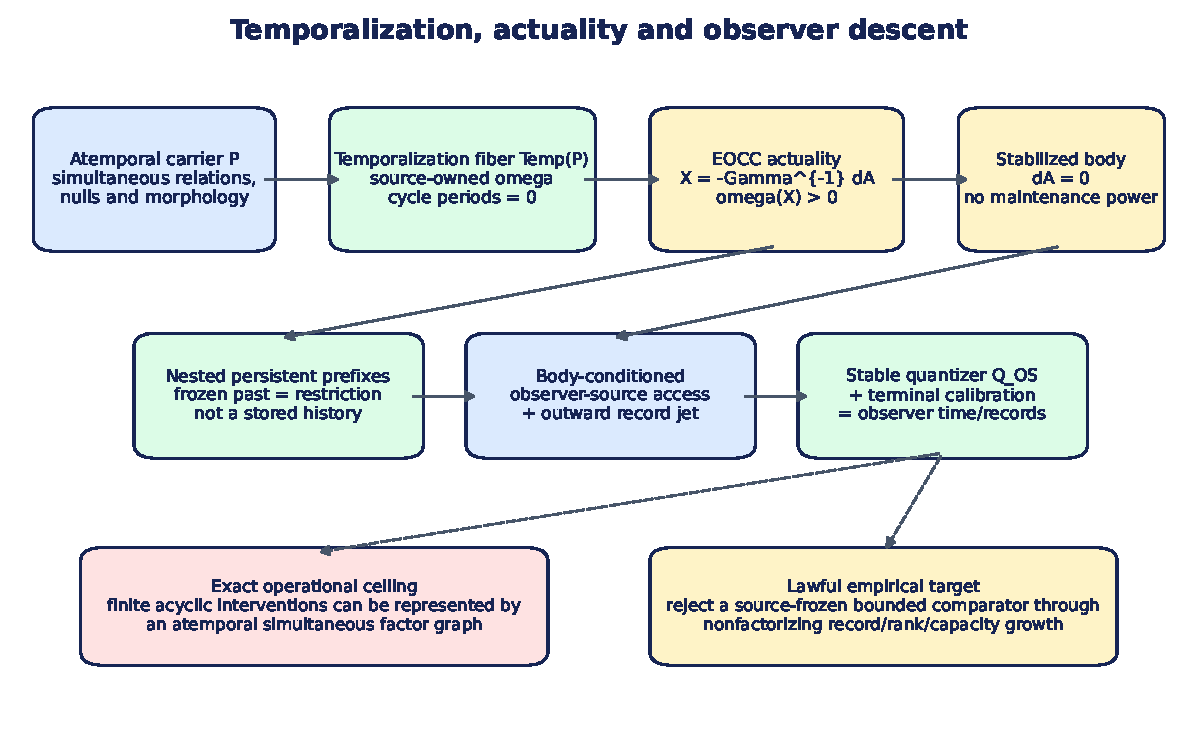
\includegraphics[width=\linewidth]{figures/fig_temporalization_proof_spine.pdf}
\caption{Temporalization and observer descent.  The upper row separates an
atemporal carrier, an integrable order structure, EOCC actuality and the
stabilized endpoint.  The middle row shows persistent prefixes and resolved
observer records.  The lower row records the operational ceiling and the
only lawful empirical comparison.}
\label{fig:proof-spine}
\end{figure}

\section{Morphogenesis, progressive stabilization and the frozen past}

\subsection{The base executes a seed-owned relational program}

The current synthesis assigns distinct roles:
\begin{equation}
 \boxed{\begin{gathered}
 \text{seed: generative relational key},\qquad
 \text{base: susceptibility and response},\\
 \text{body: realized stable response}
 \end{gathered}}
 \label{eq:role-split}
\end{equation}
A representative local response law is
\begin{equation}
 \Gamma(M)\dot M=-D_M\mathcal A_{B,s_U}(M).
 \label{eq:formation-law}
\end{equation}
This does not place a material seed next to a distant front.  The fixed seed
acts through its representation in the already realized body and the
base-owned local relation law.  A formed prefix can therefore mediate access
to the next admissible relation without the original seed being spatially
adjacent to that front.  The analogy to a signal traversing a network is only
safe after one states which invariant the network preserves.

The relay result is asymmetric.  A protected motif or relation class can be
transported through lossy local maps and remain coherent by induction.  But
attenuation alone does not choose between smaller subsequent changes and
longer delays.  In a linear zero-threshold response it can reduce amplitude
while leaving a normalized relaxation time unchanged.  Genuine slowdown
requires an additional source-owned mechanism such as cumulative body-additive
drag, a moving minimum, differentiated response modes or a threshold.  Pure
edge-difference damping is an exact same-stiffness control that need not slow
with depth.

\subsection{Progressive hardening is weaker than exact freezing}

Let \(P_a\) denote the realized prefix below progress level \(a\).  The
coherent-extension law is
\begin{equation}
 a\le b\Longrightarrow P_a\subseteq P_b,
 \qquad
 \operatorname{Res}_{ba}(M_b)=M_a.
 \label{eq:prefix-persistence}
\end{equation}
This is the precise content of a body becoming rigid toward the past.  It
does not require a stored history.  Earlier relations persist as restrictions
of the later compatible body.

Exact finite-parameter freezing is nongeneric for smooth positive gradient
flows; a regular solution often approaches equilibrium asymptotically.
Operational freezing is weaker and sufficient.  If a stable observer cell
cannot distinguish \(M(\sigma)\) from \(M_*\), then a finite cell-entry
parameter exists even when exact equality occurs only at infinity.  In the
linear scalar control
\begin{equation}
 q(\sigma)-q_*=(q_0-q_*)e^{-\sigma/\tau_{\rm rel}},
 \label{eq:linear-relaxation}
\end{equation}
the resolved stabilization parameter scales as
\begin{equation}
 \sigma_{OS}^{\rm stab}
 =\tau_{\rm rel}\log{\|q_0-q_*\|\over\delta_{OS}}+O(1),
 \label{eq:resolution-freeze}
\end{equation}
where \(\delta_{OS}\) abbreviates a source-owned stable-cell scale rather
than defining readout equivalence by a nontransitive distance threshold.
Thus a coarse observer can see a frozen body while a finer observer still
resolves residual formation.

\subsection{No passive maintenance power at the endpoint}

Along EOCC,
\begin{equation}
 {d\mathcal A_{\rm occ}\over d\sigma}
 =-\left\langle d\mathcal A_{\rm occ},
 \Gamma^{-1}d\mathcal A_{\rm occ}\right\rangle.
 \label{eq:lyapunov}
\end{equation}
If the body is a joint stable minimum of the base and seed, the endpoint has
zero response current.  The persistent seed is therefore best interpreted as
a relational asymmetry defining the minimum, not a fuel packet consumed to
hold the finished body in place.  Action is exchanged or dissipated during
formation and rearrangement; a static stable endpoint need not require
continuous power.  Removing or changing the seed may move the minimum and
restart response, but that is a different intervention.

\section{Observer time, resolved records and history refinement}

\subsection{A continuous precursor is not yet an operational tick}

Let \(\mathcal R_{OS}\) be the complete source-frozen record descriptor and
let \(C_0\) be the stable quantizer cell containing the zero precursor.  On a
local formation segment \(d(\delta)\), suppose
\begin{equation}
 \mathcal R_{OS}(d(\delta))-\mathcal R_{OS}(0)
 =\delta a+\eta(\delta),
 \qquad \|\eta(\delta)\|\le {C\over2}\delta^2.
 \label{eq:record-jet}
\end{equation}
If \(B_{r_-}\subseteq C_0\subseteq B_{r_+}\), then
\begin{align}
 \delta\|a\|+{C\over2}\delta^2<r_-
 &\Longrightarrow Q_{OS}(d(\delta))=Q_{OS}(0),
 \label{eq:unresolved-cell}\\
 \delta\|a\|-{C\over2}\delta^2>r_+
 &\Longrightarrow Q_{OS}(d(\delta))\ne Q_{OS}(0).
 \label{eq:resolved-cell}
\end{align}
These Paper-VI results are imported to make one point: a nonzero Parent or
channel derivative need not be a resolved observer transition.  Time
quantization is the smallest transition resolved by this observer--source
instrument and context, not a universal atom of parent time.

On a constant-rank access stratum, only the outward Kato projector jet moves
the accessible subspace.  A complete exhaustive effect--Choi instrument
detects every nonzero outward jet in at least one Choi record, while immediate
effect probabilities and incomplete record subsets can remain blind.  This
is why an empirical temporal test must freeze the complete instrument rather
than choose a favorable terminal after seeing the data.  Kato perturbation
theory supplies the standard mathematical control on the projector motion
\citep{Kato1995}.

\subsection{History refinement without a Parent history store}

Let \((\mathcal P,\mu)\) be one source-frozen atemporal Parent ensemble and
let \(X_a\) and \(D_b\) be simultaneous early and later record maps.  The
observer-relative compatible classes satisfy
\begin{equation}
 \mathcal H_{x,d}^{(a,b)}
 =X_a^{-1}(x)\cap D_b^{-1}(d)
 \subseteq X_a^{-1}(x)=\mathcal H_x^{(a)}.
 \label{eq:history-refinement}
\end{equation}
This is refinement by intersection, not later rewriting of an earlier Parent
state.  Stable record invariance alone is weaker than no-signalling.  If the
pre-choice weight \(\mu\) is common to all later settings and the later
instrument is represented by a normalized kernel \(K_b(d|p)\), then
\begin{equation}
 \sum_dP(x,d|a,b)
 =\int_{\mathcal P}{\bf1}_{X_a(p)=x}\,d\mu(p)
 =P(x|a),
 \label{eq:no-retro}
\end{equation}
independently of \(b\).  Conditioning on \(d\) may reveal different
subensembles without creating a signal to the earlier observer.  Delayed-choice
and eraser-type statistics therefore fit Parent-fiber refinement but do not
prove Tau Core.

\subsection{Positive proto-order and negative weak times}

A post-selected weak-time quantity may be negative even when the underlying
actual response order is positive.  The observer quantity depends on
preparation, interference and postselection, schematically
\begin{equation}
 T_{\rm weak}=F(\text{interaction},\text{preselection},\text{postselection}),
 \label{eq:weak-time}
\end{equation}
whereas \(\omega_{\rm occ}(X_{\rm EOCC})>0\) concerns the Parent formation
packet.  A finite compatibility witness exists because conditional
quasi-averages need not be positive durations.  This is consistent with weak
measurement theory \citep{Aharonov1988}; it is not evidence for a Tau-specific
deviation or backwards Parent time.

\subsection{Record persistence is not an entropy arrow}

The occurrence action, observer order and entropy are different typed
objects.  For a differentiable parent lift
\(\mathcal S_P=\mathcal S_O\circ Q_{OS}\), EOCC gives
\begin{equation}
 {d\mathcal S_P\over d\sigma}
 =-\left\langle d\mathcal S_P,
 \Gamma^{-1}d\mathcal A_{\rm occ}\right\rangle.
 \label{eq:entropy-action-rate}
\end{equation}
Consequently the exact local alignment condition for nondecreasing
\(\mathcal S_P\) is
\begin{equation}
 \boxed{
 \left\langle d\mathcal S_P,
 \Gamma^{-1}d\mathcal A_{\rm occ}\right\rangle\le0.}
 \label{eq:entropy-alignment}
\end{equation}
Equation~\eqref{eq:entropy-alignment} is necessary and sufficient locally,
but it is not implied by action descent.  Two entropy functions with opposite
gradients along the same EOCC orbit give opposite entropy arrows while
preserving the action, occurrence order and stable-record packet.  Thus the
identification \(\mathcal S_P=-\mathcal A_{\rm occ}+\mathrm{const}\) is a
possible completion, not a thermodynamic derivation.

There is nevertheless an exact readout-level result.  Let \(Y_n\) be the old
resolved classes and suppose the one complete later readout has the
source-frozen non-erasing form
\begin{equation}
 Y_{n+1}=\coprod_{y\in Y_n}\{y\}\times F_y,
 \qquad c_n(y,f)=y,
 \label{eq:visible-refinement}
\end{equation}
with a consistent ensemble
\begin{equation}
 p_n(y)=\sum_{f\in F_y}p_{n+1}(y,f).
 \label{eq:refinement-marginal}
\end{equation}
The Shannon chain rule then yields
\begin{equation}
 \boxed{H(Y_{n+1})-H(Y_n)=H(F_n\mid Y_n)\ge0.}
 \label{eq:readout-entropy-increment}
\end{equation}
The inequality is strict exactly when the new front effect resolves variation
hidden inside at least one old class.  If \(Q_n\) is the old quantizer and
\(f_n\) the relative new effect, the exact finite criterion is
\begin{equation}
 \exists x,x':\quad Q_n(x)=Q_n(x'),\qquad f_n(x)\ne f_n(x').
 \label{eq:front-nonfactorization}
\end{equation}
On a regular smooth stratum this becomes
\begin{equation}
 \operatorname{rank}\!\begin{bmatrix}DQ_n\\Df_n\end{bmatrix}
 >\operatorname{rank}DQ_n,
 \qquad
 \ker DQ_n\not\subseteq\ker Df_n.
 \label{eq:front-rank-novelty}
\end{equation}
These are imported net results of the morphogenesis program; their detailed
finite controls remain with the canonical source.  They prove accessible
readout refinement, not creation of new Parent information.  Indeed a finer
observer can have increasing \(H(Y_n)\) while its loss
\(H(X\mid Y_n)\) decreases.  Neither quantity is automatically physical
thermodynamic entropy.  That promotion still requires a source-owned
macroterminal, conserved quantities, an equilibrium measure and a standard
thermodynamic limit; see the standard information-theoretic distinction in
\citet{CoverThomas2006}.

The corrected arrow statement is therefore conditional:
\begin{equation}
 \boxed{\begin{gathered}
 \text{odd source orientation}+\text{EOCC actuality}
 +\text{persistent records}\\
 +\text{non-erasing visible refinement}+\text{consistent ensemble}
 +\text{thermodynamic identification}\\
 \Longrightarrow
 \text{aligned actuality, record and thermodynamic arrows}.
 \end{gathered}}
 \label{eq:arrow-alignment-packet}
\end{equation}
The present source packet does not derive the last three physical premises or
the low-entropy boundary.  Hence this composition does not solve the Past
Hypothesis; it isolates what a Tau-side solution would still have to own.

\subsection{Common ownership no-go and minimal free-action completion}

Even one source packet owning the occurrence law and the complete readout does
not fix the entropy sign.  At an occupied point in $X=\mathbb R^2$, choose
\begin{equation}
 \mathcal A=x_1+\tfrac12x_2^2,\qquad
 Q=x_1,\qquad f=x_2,\qquad \Gamma=I.
 \label{eq:common-source-countermodel}
\end{equation}
Then $X_{\rm EOCC}=-e_1$, while
$\ker DQ=\operatorname{span}(e_2)$ and $Df(e_2)=1$, so the same packet has
strict hidden-fiber front novelty.  Nevertheless the two scalar terminals
$\mathcal S_+=-x_1$ and $\mathcal S_-=x_1$ give
\begin{equation}
 d\mathcal S_+(X_{\rm EOCC})=+1,\qquad
 d\mathcal S_-(X_{\rm EOCC})=-1.
 \label{eq:common-source-opposite-arrows}
\end{equation}
Thus common ownership, EOCC and front nonfactorization do not entail a
thermodynamic arrow.

A sufficient completion is source-owned free-action structure
\begin{equation}
 \mathcal A_{\rm occ}=\mathcal E_P-\Theta_P\mathcal S_{\rm th},
 \qquad \Theta_P>0,\qquad
 d\mathcal E_P(X_{\rm EOCC})=d\Theta_P(X_{\rm EOCC})=0.
 \label{eq:free-action-source-law}
\end{equation}
Combining Eq.~\eqref{eq:free-action-source-law} with EOCC yields
\begin{equation}
 \boxed{
 {d\mathcal S_{\rm th}\over d\sigma}
 ={1\over\Theta_P}
 \left\langle d\mathcal A_{\rm occ},
 \Gamma^{-1}d\mathcal A_{\rm occ}\right\rangle\ge0,}
 \label{eq:free-action-entropy-theorem}
\end{equation}
strictly away from equilibrium.  Conservation is essential: if
$d\mathcal E_P(X_{\rm EOCC})$ is sufficiently negative, the entropy rate
reverses while EOCC still descends.  The discrete front result becomes
thermodynamic under the stronger optional macroterminal identity
\begin{equation}
 \mathcal S_{{\rm th},n+1}-\mathcal S_{{\rm th},n}
 =k_BH(F_n\mid Y_n)+\Sigma_n,\qquad \Sigma_n\ge0.
 \label{eq:front-macroterminal-identity}
\end{equation}
Equations~\eqref{eq:free-action-source-law} and
\eqref{eq:front-macroterminal-identity} are additional enriched source laws,
not consequences of common source naming.  The latter is sufficient, not
necessary.  Current Tau has not derived their
physical ownership, the equilibrium measure defining
$\mathcal S_{\rm th}$, or the initial low-entropy boundary.

\subsection{Configuration-Laplacian free action and the front-entropy no-go}

The conserved-macrofiber program supplies a weaker and more natural positive
route.  On a connected finite configuration carrier
$\Sigma_m=\{1,\ldots,N\}$, let
\begin{equation}
 (Lp)_i=\sum_jw_{ij}(p_i-p_j),\qquad
 w_{ij}=w_{ji}\ge0,qquad u_i=N^{-1}.
 \label{eq:configuration-laplacian}
\end{equation}
For positive $p$, define the logarithmic mean
\begin{equation}
 \Lambda(a,b)=\frac{a-b}{\log a-\log b},\qquad
 \Lambda(a,a)=a,
 \label{eq:logarithmic-mean}
\end{equation}
and the positive Onsager operator
\begin{equation}
 (\mathsf K_p\xi)_i
 =\sum_jw_{ij}\Lambda(p_i,p_j)(\xi_i-\xi_j).
 \label{eq:onsager-operator}
\end{equation}
With
\begin{equation}
 \mathcal A_{\rm th}(p)=\vartheta D(p\Vert u),\qquad
 \Gamma_p^{-1}=\vartheta^{-1}\mathsf K_p,
 \label{eq:thermal-occurrence-action}
\end{equation}
the identity
$\Lambda(p_i,p_j)(\log p_i-\log p_j)=p_i-p_j$ gives
\begin{equation}
 \boxed{\dot p=-\Gamma_p^{-1}d\mathcal A_{\rm th}=-Lp.}
 \label{eq:laplacian-eocc}
\end{equation}
Thus symmetric macrofiber mixing is exactly an EOCC gradient flow under the
source-derived logarithmic-mean mobility.  Setting
\begin{equation}
 \mathcal S_{\rm th}=k_BH(p),\qquad
 T_P=\vartheta/k_B,\qquad
 \mathcal E_m=\vartheta\log N,
 \label{eq:thermal-terminals}
\end{equation}
yields
\begin{equation}
 \boxed{\mathcal A_{\rm th}=\mathcal E_m-T_P\mathcal S_{\rm th}}
 \label{eq:derived-free-action}
\end{equation}
and
\begin{equation}
 \boxed{
 {d\mathcal S_{\rm th}\over d\sigma}
 ={k_B\over2}\sum_{i,j}w_{ij}(p_i-p_j)
 (\log p_i-\log p_j)\ge0.}
 \label{eq:laplacian-entropy-production}
\end{equation}
Equality holds only at the uniform state on a connected carrier.  This is the
infinitesimal form of the conditional macrofiber H-theorem already owned by
the foundation program.

The global occurrence action can be restricted to
$\mathcal A_{\rm th}$ only if one physical incidence identifies the occupied
temporal front with this same conserved configuration carrier and its positive
activation.  The present configuration-graph and convex-weight packets make
that construction nonempty, but do not prove the identification.

Nor does Eq.~\eqref{eq:front-macroterminal-identity} follow.  At equilibrium
on a uniform two-state carrier, thermal mixing gives
$\Delta\mathcal S_{\rm th}=0$.  A constant old readout and a new front label
that distinguishes the two states gives $H(F\mid Y)=\log2>0$.  The carrier
and measure can be common, yet the proposed identity would require
$\Sigma=-k_B\log2<0$.  Therefore accessible front refinement and
thermodynamic production may share a source and orientation without having
equal increments.  The remaining physical target is one front-to-
configuration incidence, not FMT-P1.

That target is not already implied by the two existing packets.  Keep fixed
the complete seed--base response reduct and a two-state symmetric thermal
carrier with positive activation.  One extension identifies the two front
labels bijectively with the two thermal configurations.  A second extension
keeps every upstream object fixed but admits only the constant incidence from
both front labels to one thermal state.  A complete two-label front readout
cannot factor through that rank-one incidence.  Hence
\begin{equation}
 \boxed{
 \mathrm{SBMR+configuration\ heat}
 \not\Longrightarrow \mathrm{front\!\!-configuration\ incidence}.}
 \label{eq:tfci-non-entailment}
\end{equation}
The conclusion remains true after positive thermal activation is supplied;
the missing datum is cross-typed registration rather than a rate.

A minimal positive completion is exact.  Let one primitive source alphabet
$\mathcal A_{\rm src}$ carry source-owned bijections
\begin{equation}
 e_F:\mathcal A_{\rm src}\overset{\sim}{\longrightarrow}F,
 \qquad
 e_\Sigma:\mathcal A_{\rm src}\overset{\sim}{\longrightarrow}\Sigma_m,
 \qquad
 \chi=e_\Sigma e_F^{-1}.
 \label{eq:tfci-common-atom}
\end{equation}
If their pullbacks agree on the complete macroterminal, measure and local
rewrite incidence, $\chi$ is the unique incidence with those properties.
Positive source depth $u$ additionally gives
$\lambda(u)=2u/\ell_*>0$ under the existing positive-mode depth calibration.
This proves the common-carrier arrow alignment conditionally.  The current
Tau source inventory does not derive the primitive atomic co-ownership in
Eq.~\eqref{eq:tfci-common-atom}; equal cardinality or common source naming is
insufficient.

Nor does one universal seed force that premise.  Grant the one structured
seed the split algebra
\begin{equation}
 \mathcal A_U=\mathbb Rp_0\oplus\mathbb Rp_1,
 \qquad p_ap_b=\delta_{ab}p_a,
 \qquad p_0+p_1=1.
 \label{eq:universal-seed-split-algebra}
\end{equation}
Keep the front action faithful,
$\rho_F(p_0)=\operatorname{diag}(1,0)$ and
$\rho_F(p_1)=\operatorname{diag}(0,1)$.  The same one-seed reduct admits both
the matching faithful thermal action $\rho_\Sigma^+=\rho_F$ and the unital
nonfaithful action
\begin{equation}
 \rho_\Sigma^-(p_0)=I_2,
 \qquad \rho_\Sigma^-(p_1)=0.
 \label{eq:universal-seed-nonfaithful-control}
\end{equation}
Both may carry the same two-state thermal Laplacian, measure and positive
activation.  The second action collapses one primitive seed atom and cannot
support atomic co-ownership.  Thus universal-seed uniqueness is insufficient
even after a primitive algebra is supplied.

The corrected sufficient theorem is finite.  If a split algebra with $N$
primitive idempotents acts faithfully, unitally and multiplicity-freely on
both $V_F$ and $V_\Sigma$, with
$\dim V_F=\dim V_\Sigma=N$, then its pairwise orthogonal nonzero primitive
projectors have positive integer ranks summing to $N$.  Every rank is
therefore one.  The common primitive spectrum consequently fixes exactly one
front atom and one thermal atom per idempotent, and hence fixes their
incidence up to simultaneous algebra relabeling.  If the measure,
macroterminal and rewrite graph also live on that primitive spectrum,
Eq.~\eqref{eq:tfci-common-atom} and the conditional arrow alignment follow.
The existing PUSC structure is a candidate primitive algebra, but the two
physical faithful module actions and common primitive rewrite ownership are
not yet derived.

These representation premises admit a sharper source-side compression.  Let
$\mathcal A_U\cong\mathbb R^N$ act unitally on an $N$-dimensional carrier
$V_X$, and let a source-descended root $v_X$ define
\begin{equation}
 C_X:\mathcal A_U\longrightarrow V_X,
 \qquad C_X(a)=\rho_X(a)v_X.
 \label{eq:cyclic-source-evaluation}
\end{equation}
If $v_X$ is cyclic, $C_X$ is onto and hence an isomorphism.  Therefore
$\rho_X$ is faithful.  Moreover the vectors $C_X(p_a)$ form a basis and
$\operatorname{im}\rho_X(p_a)=\mathbb R C_X(p_a)$, so every primitive atom
occurs exactly once.  Applied separately to the front and thermal carriers,
paired cyclicity replaces faithfulness, multiplicity freedom and atomic
exhaustivity by the single certificate
\begin{equation}
 \gamma_{\rm pair}
 =\min_{X\in\{F,\Sigma\}}
 \lambda_{\min}(C_X^*C_X)>0.
 \label{eq:paired-cyclic-gram}
\end{equation}
Together with the common primitive measure, macroterminal and rewrite graph,
this condition implies the unique incidence in
Eq.~\eqref{eq:tfci-common-atom}.  It is not implied by common ancestry.  In
the control of Eq.~\eqref{eq:universal-seed-nonfaithful-control}, choose
$v_F=(1,1)^T$ and $v_\Sigma=(1,0)^T$.  Then $C_F=I_2$ but
$C_\Sigma=\operatorname{diag}(1,0)$, so the same seed algebra has a cyclic
front root and a singular thermal root.  The current protected-parent
cyclicity result therefore supplies a template, not a proof that both
post-body descents preserve cyclicity.

The primitive joint Hessian now makes the source origin of this condition
explicit.  After body stabilization, let $E_U$ carry a positive source metric
$K_U$, let $H_X>0$ be the front or thermal response Hessian, and let $B_X$ be
the mixed seed--carrier block.  The quadratic two-jet
\begin{equation}
 \mathcal A_X(a,z_X)=\tfrac12 z_X^*H_Xz_X-z_X^*B_Xa
 +\tfrac12a^*K_Ua
 \label{eq:primitive-paired-work-action}
\end{equation}
gives, by stationarity,
\begin{equation}
 C_X=H_X^{-1}B_X,
 \qquad W_X=C_X^*H_XC_X=B_X^*H_X^{-1}B_X.
 \label{eq:primitive-paired-work-gram}
\end{equation}
Positivity of $H_X$ implies
$\ker W_X=\ker B_X=\ker C_X$.  Therefore paired cyclicity is equivalent to
\begin{equation}
 \ker B_F=\ker B_\Sigma=\{0\}.
 \label{eq:paired-mixed-block-injectivity}
\end{equation}
The metric form
$W_X\succeq\epsilon_XK_U$ with $\epsilon_X>0$ gives the explicit bound
\begin{equation}
 \gamma_{\rm pair}\ge
 \min_X\frac{\epsilon_X\lambda_{\min}(K_U)}
                 {\lambda_{\max}(H_X)}>0.
 \label{eq:paired-work-lower-bound}
\end{equation}
Equivalently, if one full-rank master coupling $B_U$ is followed by
$B_X=T_XB_U$, it is sufficient that
$\ker T_X\cap\operatorname{im}B_U=\{0\}$ on both legs.  This is protected
non-erasure, not global losslessness.

Neither stability nor combined completeness forces this result.  Taking
$K_U=H_F=H_\Sigma=I_2$, $B_F=I_2$ and
$B_\Sigma=\operatorname{diag}(1,0)$ leaves both carrier Hessians positive and
the stacked coupling full rank, while the thermal work Gram is singular.
Thus a stable thermal response may remain blind to one seed atom.  The exact
common-unit identity $W_F=W_\Sigma=K_U$ is a sufficient source/root
Gram-isometry completion, but the current Tau action does not derive it for
these two typed carriers.

The zero-kernel requirement is stronger than necessary for a lossy Tau
descent.  Put $K_F=\ker B_F$ and $K_\Sigma=\ker B_\Sigma$.  A quotient
$E_U/K$ admits well-defined and faithful induced maps on both carriers if and
only if
\begin{equation}
 K_F=K_\Sigma=:K_{\rm com}.
 \label{eq:common-kernel-descent}
\end{equation}
Indeed, descent requires $K\subseteq K_X$, whereas faithfulness requires
$K_X\subseteq K$.  Thus $E_U/K_{\rm com}$ is the unique maximal common
faithful source quotient.  A zero common kernel gives complete universal-seed
alignment.  A nonzero common kernel gives only quotient-level alignment unless
the erased sector is proved null for every claimed macroterminal.

Equal ranks do not suffice.  The pair
$B_F=\operatorname{diag}(1,0)$,
$B_\Sigma=\operatorname{diag}(2,0)$ has one faithful common quotient, while
$B_F=\operatorname{diag}(1,0)$,
$B_\Sigma=\operatorname{diag}(0,1)$ has equal ranks but different kernels.
Both can descend from the same injective master body coupling.  Consequently,
even if every seed atom is essential to formation of the complete body,
lossy post-body descents need not erase the same atoms.  The least physical
completion is common protected-kernel descent, not universal losslessness.

\section{Operational equivalence and the limit of finite experiments}

\subsection{Finite interventional simulation no-go}

Let \(G=(V,E)\) be a finite acyclic graph with local response laws
\begin{equation}
 x_v=f_v^{i_v}(x_{\operatorname{Pa}(v)},\xi_v),
 \label{eq:dag-process}
\end{equation}
including predeclared interventions, adaptive decision nodes and shared
exogenous variables.  The simultaneous relation
\begin{equation}
 \mathcal S_i=\left\{(x,\xi):
 x_v-f_v^{i_v}(x_{\operatorname{Pa}(v)},\xi_v)=0
 \ \forall v\right\}
 \label{eq:simultaneous-factor}
\end{equation}
has the same deterministic solutions.  For stochastic kernels, the product
\begin{equation}
 \mu_i(dx)=\prod_{v\in V}
 K_v^{i_v}(dx_v\mid x_{\operatorname{Pa}(v)})
 \label{eq:kernel-factorization}
\end{equation}
is both the sequential sampling law and the atemporal factor-graph law.
Shared exogenous variables preserve the counterfactual coupling.  Hence every
terminal and joint table in this class agrees.

The result resembles standard equivalence issues in causal modeling
\citep{Pearl2009}, but its role here is ontological discipline: manipulating
an internal process does not prove that the Parent literally traverses the
algorithm used to generate the same table.  The simultaneous representation
is not a memory store or an instruction to run a solver in hidden time.

\subsection{What can still be tested}

The no-go does not make the temporal completion scientifically empty.  It
changes the admissible null hypothesis.  A decisive class-relative test must
freeze before endpoint inspection:
\begin{enumerate}[label=(D\arabic*)]
\item a source-complete bounded atemporal comparator \(\mathcal C_A\);
\item a temporal completion \(\mathcal C_T\) with no post-result source or
      access enlargement;
\item one common intervention cut and complete observer instrument;
\item nuisance, wrong-family and contextual-access controls;
\item an observable whose prediction sets are disjoint or whose complete
      response rank exceeds the frozen operational capacity of
      \(\mathcal C_A\).
\end{enumerate}

One local linear form is
\begin{equation}
 \Delta r_k
 =\rank\begin{pmatrix}J_{\rm old}\\J_k\end{pmatrix}
  -\rank(J_{\rm old}),
 \label{eq:rank-innovation}
\end{equation}
after quotienting standard nuisance tangents and freezing the common cut.
Positive prefix rank growth rejects only a comparator whose complete effect
module has been bounded independently.  An unrestricted contextual
atemporal descriptor can add a separate context sector and saturate any finite
table.  Calling that unrestricted class ``falsified'' would merely punish it
for not being the bounded model that was tested.

\begin{proposition}[Empirical proof ceiling]
Finite terminal agreement or disagreement can select between predeclared
bounded model classes.  It cannot by itself prove literal Parent traversal
against the unrestricted atemporal class containing the projected temporal
completion.  Nature-level temporal evidence requires both a source-derived
comparator-capacity restriction and a terminal effect that survives the full
observer/source/nuisance quotient.
\end{proposition}

This proposition is a synthesis of the finite saturation, common-cut and
source-cost results.  It prevents the atemporal model from becoming an
unfalsifiable ``anything fits'' explanation while also preventing an
artificially weak comparator from manufacturing temporal evidence.

\section{Formation budget, four-dimensional exchange and dark-sector limits}

\subsection{Finite parent-action budget}

For a regular EOCC section ending at a stable minimum,
\begin{equation}
 \Delta\mathcal A_{\rm form}
 =\mathcal A_{\rm occ}(q_0)-\mathcal A_{\rm occ}(q_*)
 =\int d\sigma\,
 \left\langle d\mathcal A_{\rm occ},
 \Gamma^{-1}d\mathcal A_{\rm occ}\right\rangle.
 \label{eq:formation-budget}
\end{equation}
This is an exact parent-action identity inside the working completion.  It is
not yet energy in joules, a local density or stress-energy.  The conversion
requires a terminal metric, time direction, field normalization and action
unit.  These belong downstream and may not be chosen from a dark-sector fit.

\subsection{One exact conditional 4D soldering}

As a nonempty terminal completion, introduce positive scales
\begin{equation}
 t=t_*\sigma,
 \qquad \varphi=\varphi_*q,
 \qquad V(\varphi)=\varepsilon_*\mathcal A_{\rm occ}(q),
 \label{eq:unit-soldering}
\end{equation}
and a future timelike terminal vector \(u^\mu\).  The first-order law
\begin{equation}
 \Upsilon D_t\varphi+V_{,\varphi}=0
 \label{eq:4d-formation-law}
\end{equation}
can reproduce the scalar EOCC orbit for a corresponding positive
\(\Upsilon\).  The algebraic form stress
\begin{equation}
 T_{\mu\nu}^{\rm form}=-Vg_{\mu\nu}
 \label{eq:form-stress}
\end{equation}
is not separately conserved during formation:
\begin{equation}
 \nabla_\mu T_{\rm form}^{\mu\nu}
 =J_{\rm form}^{\nu}
 =-V_{,\varphi}\nabla^\nu\varphi.
 \label{eq:exchange-current}
\end{equation}
Bianchi compatibility requires a receiver with
\begin{equation}
 \nabla_\mu T_{\rm res}^{\mu\nu}=-J_{\rm form}^{\nu}.
 \label{eq:receiver}
\end{equation}
The integrated transfer equals \(\varepsilon_*\Delta\mathcal A_{\rm form}\)
under this soldering, but the three conversion scales remain free upstream.

\subsection{Why this does not derive dark matter or dark energy}

The same homogeneous positive source
\(S(t)=\Upsilon\dot\varphi^2\) admits receiver equations
\begin{equation}
 \dot\rho_w+3H(1+w)\rho_w=S(t)
 \label{eq:receiver-family}
\end{equation}
for \(w=-1,0,1/3\), giving vacuum-like, dust-like and radiation-like
backgrounds.  Conservation therefore fixes loading but not pressure, sound
speed, anisotropic stress, localization, clustering or the split among
receivers.  The scalar formation packet supplies no unique halo, lensing or
cosmological-constant prediction.

Moreover, an atemporal completed-orbit model with the same restricted orbit
and terminal soldering reproduces
\((\varphi,T_{\mu\nu}^{\rm form},J_{\rm form}^\nu)\).  The conditional 4D
exchange current is therefore not an actuality-nonfactorizing discriminator.
The robust conclusion is narrower:
\begin{quote}
Temporal formation can conditionally source a finite 4D exchange packet, but
neither its observed existence nor its total budget proves Parent temporality
or selects a dark sector.
\end{quote}

\section{Observational program and preserved negative results}

The temporal program inspected several public-data families.  None currently
crosses the source-to-terminal and comparator-capacity gates.  Table
\ref{tab:data-status} records the net status rather than retelling every
preflight.

\begin{table}[t]
\centering
\small
\begin{tabularx}{\linewidth}{L{0.21\linewidth}L{0.32\linewidth}X}
\toprule
Family & What was obtained & Current temporal verdict \\
\midrule
Resolved galaxy morphology/age & Frozen clock-blind geometry, null or
ordinary-evolution-compatible endpoints, source-label and covariance audits &
No formation-specific temporal signal; later terminal selection forbidden \\
Atomic and many-body ramps & Stage-resolved or return-path method preflights &
Useful controls, but no Parent bridge and no temporal discrimination \\
Glass/Kovacs data & History-dependent public response with present-state
normalization controls & Public packet does not realize an identical complete
present-state comparison \\
Photonic circuits & Executable design for joint onset/coherence method
validation; partial public resources & Hardware acquisition packet, not Tau
temporality evidence \\
Quantum process/tomography tables & One centered rank-excess preflight survived
several simple nuisance projections & Broader operational cut and cross-run
replication fail; aggregate drift remains non-identifiable \\
Negative weak-time experiments & Operational example of conditioned time not
being a positive classical duration & Compatible with positive Parent order;
fully explained within standard quantum theory \\
JWST/Hubble/CMB targets & Reparameterization and sign audits & A universal
one-lapse deformation has no independent content or wrong joint sign; no Tau
signal established \\
\bottomrule
\end{tabularx}
\caption{Preserved net status of the observational program.  ``Preflight'' is
not empirical validation.  The source documents retain dataset provenance and
negative controls.}
\label{tab:data-status}
\end{table}

The strongest provisional process-tomography feature was a structured
centered rank excess in one released aggregate packet.  It did not replicate
across the wider public run family, and the released aggregates do not
identify the missing drift or context bound.  Preserving this demotion is
scientifically more valuable than treating every unexplained residual as
temporal evidence.

For cosmology, a mere reparameterization
\(t_{\rm obs}=F(\sigma)\) is physically empty unless the map changes a
source-owned relation between independently measurable sectors.  A universal
geometric lapse that gives early systems more parent formation opportunity
does not automatically have the sign required to relieve both early-structure
and late-distance tensions.  JWST, Hubble and CMB results may motivate a
future sector-specific readout law, but they do not currently select it.

\section{Proof ladder, falsification and current status}

The complete program is best summarized as a ladder.
\begin{description}[style=nextline,leftmargin=2.7cm]
\item[L0: definitions] Atemporal carrier, temporalization fiber, seed key,
observer/source quantizer and terminal maps.
\item[L1: exact finite mathematics] Cycle-period temporalizability, action
cochain exactness, positive EOCC contraction, stable-cell window, complete
record detection and no-retro marginalization.
\item[L2: conditional mechanism] One enriched seed--base/occurrence action,
positive response form, EOCC actuality, progressive stabilization and finite
formation budget.
\item[L3: physical source selection] Nature-level ownership and occupation of
the complete action, actuality law, front/access co-registration, instrument
and calibration.  This level is open.
\item[L4: empirical discrimination] Source-frozen bounded comparator,
nonfactorizing complete record and independent replication.  This level is
open.
\end{description}

The strongest current result is L2.  It is stronger than a verbal analogy:
the conditional response, order and budget are explicit and internally
audited.  It is weaker than a physical theory of time because L3 is an
additional premise and L4 has no successful endpoint.

\subsection{Failure and demotion conditions}

The temporal working completion would be weakened or rejected in its declared
domain if any of the following occurs:
\begin{enumerate}[label=(F\arabic*)]
\item the source-owned occurrence cochain has a nonzero period after the true
      physical-null quotient while the model claims one global scalar
      proto-time;
\item the proposed response metric is not positive on the retained physical
      quotient or the EOCC section fails the claimed action descent;
\item the prefix law overwrites a previously stable source-owned record;
\item the claimed observer clock depends on a nontransitive threshold rather
      than a stable quantizer partition;
\item a purported temporal signal vanishes under the complete source-owned
      instrument, wrong-family or contextual-access controls;
\item a Parent front rate is inferred from one observer tick series while the
      channel transmission or stable-cell density is fitted from that same
      series rather than frozen independently;
\item the same signal is reproduced by the predeclared bounded atemporal
      comparator without exceeding its frozen capacity;
\item a 4D energy or dark-sector claim requires an equation of state,
      localization or unit scale not derived upstream.
\end{enumerate}

Conversely, a serious strengthening would require a single source-owned
packet that simultaneously fixes the action cochain, actuality law,
formation-front/access first jet, complete record instrument and stable
quantizer, followed by an independently frozen observation exceeding a
predeclared bounded atemporal comparator.  No currently registered packet
closes that chain.

\section{Discussion}

\subsection{The body--observer metric bridge and what it does not temporalize}

The latest quantum-side audit adds one nonredundant bridge to this synthesis.
The stabilized rooted body has an inherited radial/tangential quotient metric
$K_{\rm leaf}=k_RP_R+k_TP_T$.  Exact observer compression is
\begin{equation}
 K_{{\rm occ},O}=(R_OK_{\rm leaf}^{-1}R_O^*)^{-1}.
 \label{eq:synthesis-observer-compression}
\end{equation}
This is a simultaneous body-conditioned relation, not a stored evolution.
It also does not convert the algebraic tangential rank two into a physical
two-dimensional parent surface.  A physical braid support, when present, is
an effective terminal support requiring its own topology and occupation.

The existing body and observer packets determine a canonical carrier
identification but not the projective metric ray needed to transfer stiffness.
The seed metric-copy functor (SMCF) is the minimal enriched-source postulate
that supplies this missing natural transfer for every admissible
observer--source module without placing concrete future observer values in the
universal seed.  With the isometric incidence passage it conditionally yields
\begin{equation}
 \frac{K_T^{\rm exp}}{K_R^{\rm exp}}
 =\frac{k_R}{k_T}=0.725200588341
 \label{eq:synthesis-smcf-ratio}
\end{equation}
for a calibrated static three-mode response.  One seed, common origin and the
currently proved closure conditions do not imply SMCF; a positive
metric-modulus counterfamily preserves those data while changing the ratio.
Thus the result sharpens the enriched temporal program by specifying a
source-owned body--observer handoff, but it neither proves temporal parent
traversal nor distinguishes temporal and saturated atemporal realizations by
itself.  No audited public dataset currently exposes the required source-owned
$3\times3$ susceptibility endpoint.

\subsection{Observer-dependent terminal mixing does not temporalize the Parent}

The joint-access result inherited from Papers VI and VII-A generalizes beyond
the quantum--gravity pair. For observer $O_i$, the invariant information
candidate is the complete access quotient
\begin{equation}
 X/\ker A_i,
 \qquad A_i=\bigoplus_{\alpha}T_i^\alpha,
 \label{eq:synthesis-joint-access}
\end{equation}
not an individual time, quantum, gravity, matter or radiation label. Equal
full kernels yield a unique transport between realized observer images, and
that transport may mix terminal roles on realized pure sectors. Unequal
kernels instead describe different total observer access. Across several
equal-access observers the exact transports compose as a groupoid and give
identity around a closed comparison loop.

This result is simultaneous and atemporal: it compares restrictions of one
shared parent descriptor and introduces no stored trajectory, delay history
or Parent evolution. In particular, a mode read as time by one observer and
as gravity or quantum structure by another would not prove a temporal Parent.
Conversely, terminal mixing cannot erase operational type: contextual quantum
composition cannot be fully equivalent to a classical noncontextual terminal
under a probability-preserving process equivalence. Nature-level mixing and
the physical observer family remain open.

\subsection{Internal measurement backaction does not temporalize the Parent}

A further distinction is required when the observer/apparatus is itself part
of the occupied Parent structure. After $M_\tau$ is stabilized and frozen,
let $o$ be an internal apparatus coordinate and $x$ a post-body target
coordinate in one supplied regular $C^2$ functional. Then
\begin{equation}
 D_o x_*=-H_X^{-1}C_{XO},\qquad
 D_o\Pi_a^{\rm occ}
 =D_o\Pi_a-D_x\Pi_aH_X^{-1}C_{XO}.
 \label{eq:synthesis-generalized-backaction}
\end{equation}
This is an atemporal implicit-response relation on one frozen body. It does
not introduce a Parent trajectory or identify observer time with a source
parameter. The first terminal term is direct context dependence; the second
is target-mediated backaction. Hard records require a same-context,
clamped-target comparison, so a stable output cell may hide a nonzero
continuous response and a changed context-only output need not witness
coupling. Clock, quantum, gravity and hybrid terminals are merely typed
projections of this common response, and their independent backaction content
is the rank of the stacked mediated rows. Physical source selection of
$C_{XO}$, its Nature occupation and any Tau-specific component remain open;
the observer cannot use this downstream response to reselect the body.

\subsection{Unified terminal atlas and the common immediate ancestor}

The component results imported from Papers I and VII-A assemble into one
typed master equation.  For the occupied observer--source context,
\begin{equation}
 \boxed{
 \mathfrak R_{OS}
 =
 \left\langle
  Q_{OS}^{(a)}\circ T_{OS}^{(a)}
 \right\rangle_{a\in\mathcal A_{\rm term}}
 \circ\Xi_{OS}\circ A_{OS}
 \left[
  \operatorname{Stab}_{B_\tau^{\rm base}}(\Sigma_\tau)
 \right]}
 \label{eq:synthesis-unified-terminal-atlas}
\end{equation}
collects time, quantum, gravity, matter, radiation, gauge, energy/stress and
hybrid readouts in one product codomain.  The stabilized body is the common
deep generative ancestor, while \(\Xi_{OS}\) is the common immediate
preterminal readout ancestor after irreducible observer--source access has
entered.

For any proposed terminal \(R\), descent through this ancestor is equivalent
to constancy on its fibres,
\begin{equation}
 \Xi_{OS}(x)=\Xi_{OS}(x')\Longrightarrow R(x)=R(x'),
 \qquad
 R=\bar R\circ\Xi_{OS},
 \label{eq:synthesis-ancestor-factorization}
\end{equation}
and locally implies
\(\ker D\Xi_{OS}\subseteq\ker DR\).  Equality between the ancestor kernel and
the kernel of the stacked terminal Jacobian is the exact local reconstruction
criterion.  These statements prove conditional common ancestry for the
declared occupied atlas.  They do not prove that every physically possible
Nature terminal is in that atlas.  A terminal with
\(D\Xi_{OS}v=0\) and \(DRv\neq0\) is the explicit no-bypass falsifier.

\subsection{When can the time terminal determine the other terminals?}

The common ordered distinguishability carrier must not be identified with its
clock projection. Write
\begin{equation}
 \mathfrak C_O=(\mathcal A_{OS},D_{OS},\preceq_{OS},Q_{OS}),
 \qquad
 T_O=\tau_O\circ\mathfrak C_O,
 \qquad
 F_O^\alpha=f_O^\alpha\circ\mathfrak C_O.
 \label{eq:synthesis-carrier-terminal-split}
\end{equation}
All terminals inherit one carrier, but the non-time terminals factor through
the clock exactly when the stable clock fibers equal the complete readout
fibers. For $A_O=(T_O,F_O^1,\ldots,F_O^m)$,
\begin{equation}
 \boxed{\sim_{T_O}=\sim_{A_O}.}
 \label{eq:synthesis-time-sufficiency}
\end{equation}
Locally in finite dimension this is $\ker T_O=\ker A_O$, equivalently
$\operatorname{rank}T_O=\operatorname{rank}A_O$ because $T_O$ is already one
block of the stack.

A scalar clock has rank at most one and therefore cannot determine a complete
terminal packet of rank greater than one. A multi-component time field can be
sufficient, but only if Eq.~\eqref{eq:synthesis-time-sufficiency} holds.
Local Jacobian-rank equality does not imply global nonlinear fiber equality;
$T(x)=x^2$ and a complete map also containing $F(x)=x$ give the elementary
control. In source form, with $A_O=L_AH_O^{-1}C_O$ and
$T_O=L_TH_O^{-1}C_O$, clock sufficiency is
\begin{equation}
 C_O^{-1}(H_O\ker L_T)=C_O^{-1}(H_O\ker L_A).
 \label{eq:synthesis-time-source-sufficiency}
\end{equation}
This is an additional source/exit law, not a consequence of common origin,
observer covariance or calibrated time alone.

The original intuition---a morphological body rigid toward the past and
fluid toward the future---survives in a corrected form.  ``Rigid'' means
restriction-compatible persistence of actualized prefixes and records.
``Fluid'' means the current temporalization admits more than one unresolved or
not-yet-actualized continuation at the observer's resolution.  It does not
mean that the atemporal carrier lacks all future relations, nor that a stored
past grows inside the Parent.

The seed/base analogy also survives with stricter typing.  The seed supplies
a fixed relational grammar in the language to which the base responds.  The
base supplies stiffness, susceptibility, mediation and damping structure.
Their joint law defines a stable body.  A temporal completion adds the
actuality of ordered response; it does not transform the seed into a material
energy capsule.  Instability is admissible, but our realized stable universe
selects a stable occupied branch only conditionally.

The deepest conceptual gain is the separation of four notions often called
``time'':
\begin{equation}
 \boxed{
 \text{orientation/order}
 \ne \text{actual response parameter}
 \ne \text{observer clock}
 \ne \text{SI calibration}.}
 \label{eq:four-times}
\end{equation}
Tau Core can consistently place these at different layers.  This removes the
need to put ordinary 4D time directly into the Parent, but it also prevents
the theory from claiming more than it has derived.

The entropy audit adds a parallel separation.  EOCC action descent fixes an
actuality orientation inside the adopted completion; persistent records fix a
record arrow; visible non-erasing refinement fixes an accessible-information
arrow.  A thermodynamic arrow follows only after a physical macroterminal and
its statistical-mechanical measure are derived.  Common source ownership does
not close this gap: the exact counterfamily permits opposite entropy arrows on
the same EOCC/readout/front reduct.  The free-action identity closes the local
sign only conditionally on conserved Parent energy and a positive fixed
conversion scale.  On a conserved configuration carrier the symmetric
Laplacian and logarithmic-mean mobility derive that free-action structure
exactly; the remaining issue is physical front-to-configuration registration.
The refined-front increment and thermodynamic production are distinct and
need not be equal.  A same-reduct countermodel proves that the SBMR and heat
packets do not force that registration even with positive activation.  The
unique incidence follows only under primitive atomic co-ownership of the
front and thermal presentations, which remains physically unselected.
One universal seed does not remove this premise: the same split seed algebra
admits faithful and nonfaithful thermal actions.  Faithful unital
multiplicity-free actions with dimension equal to the primitive count do
force rank-one atomic matching, but their physical ownership remains open.
Equivalently, a cyclic source root on each dimension-matched carrier forces
all three properties, and the exact paired Gram condition in
Eq.~\eqref{eq:paired-cyclic-gram} tests them without terminal entropy data.
The current action does not yet derive that both post-body source evaluations
are nonsingular.
Observer existence alone
does not choose that arrow, and record information may grow while observer
loss decreases.

The operational no-go is equally important.  If an unrestricted atemporal
model is allowed to encode an independent context for every finite experiment,
it has unlimited explanatory capacity and loses discriminatory value.  The
scientifically viable comparison is therefore not ``all atemporal structures
versus one temporal structure.''  It is a frozen, physically sourced
atemporal subclass versus a frozen temporal completion, both charged for
their source-owned operational capacity.  This is the route by which the
temporally richer but narrower model can become more predictive without being
declared true by construction.

\subsection{Common-carrier terminal overlap, phase gluing and the finite lock test}

The terminal-mixing result can now be sharpened.  Quantum effects and smeared
stress need not be independent parent substances: their gradients on one
occupied Hermitian carrier define a normalized principal-angle overlap.
Observer coarse graining contracts the effect-visible subspace, so one fixed
parent direction can become relatively gravity-dominant for a lossier
observer.  The complex structure permits this mechanism but does not select a
universal angle.

One common generating functional fixes the overlap only after its effect and
stress source directions are frozen.  If $[K,J]=0$ and $RJ=J_OR$, exact
observer compression and its spectral effects remain complex-linear, while
coframe stress is generated by the same phase-invariant functional.  Thus no
separate quantum--gravity connector is required conditionally.  Physical
occupation reduces to a body-capability/post-body-occurrence lock.  With
binary variables $q,r$, the minimal conditional law is
\[
 F_{\rm lock}(q,r)=\frac{\mathcal A_*}{2}(r-q)^2.
\]
No current declared source object derives its nonzero mixed incidence.

The exact forward discriminator uses stage $s$, independently controlled
closure permission $a$, and the solved body law $q=sa$.  It compares
$H_L:r=q$, $H_0:r=0$ and $H_P:r=s$.  The closure-allowed post cell separates
$H_L$ from $H_0$, while the closure-blocked post cell separates $H_L$ from
$H_P$ whenever the calibrated phase proxy is informative.  Omitting either
cell produces an exact model equivalence.  Direct actuator leakage is
confounded with mediation and requires a transportable matched dummy.  This
protocol can test the declared incidence but cannot distinguish temporal
Parent traversal from an atemporal completed descriptor carrying the same
controlled relations.

\subsection{Full-4D standard-excess boundary}

The temporal readout assembled here is one terminal image of a possible
observer-specific full-4D metric excess.  The exact parent-side comparison is
\[
 E_K=(K_{HH}-K_{\rm std})-CK_{VV}^{-1}C^\dagger,
\]
not the positive Schur term alone.  Since \(C\neq0\) is compatible with
\(E_K=0\), observer-relative clock variation cannot be inferred from parent
mixing alone.  A physical test must freeze the common \(E_g\), map it through
clock and co-owned non-temporal terminals, quotient duplicate information and
retain the full joint covariance.  This synthesis imports that scoring
boundary but does not claim a nonzero occupied packet.

\section{Graph/Hilbert temporalization boundary}

The conditional Gram formulation clarifies rather than removes the
atemporal/temporal distinction.  Given source-owned probes, a common unitary
motion of all rays leaves every overlap invariant:
\begin{equation}
 |\chi_a(\lambda)\rangle=U(\lambda)|\chi_a(0)\rangle
 \quad\Longrightarrow\quad
 G_{ab}(\lambda)=G_{ab}(0).
 \label{eq:synthesis-common-unitary-gram}
\end{equation}
Consequently a sequence of Gram matrices cannot detect a global unitary
Parent motion.  A change in $G$ records only relative transport, a changed
state, a nonunitary restriction or a changed observer--source context.  None
of those possibilities by itself proves fundamental Parent evolution.

The Fubini--Study distance between rays is likewise only a dimensionless
metric.  It supplies no preferred orientation, event order, rate or unit.
Observer time emerges only after the atemporal body-conditioned channel has
provided an integrable ordered carrier, a stable source-derived quantizer and
a calibrated clock pairing.  Hence
\begin{equation}
 d_{\rm FS}\not\equiv\Delta t_O
 \label{eq:synthesis-fs-no-clock}
\end{equation}
without those extra physical structures.

This yields the strict synthesis
\begin{equation}
 \begin{gathered}
 \text{atemporal source/body relations}
 \longrightarrow\text{conditional projective readout geometry}\\
 \longrightarrow\text{ordered observer-relative classes}
 \longrightarrow t_O,\\
 \text{projective geometry}
 \not\Longrightarrow
 \text{a Parent trajectory or stored history}.
 \end{gathered}
 \label{eq:synthesis-gram-placement}
\end{equation}
The temporal branch is therefore retained as a temporalizable readout sector
of the atemporal architecture.  The Graph/Hilbert representation supplies
useful correlation and phase invariants, but it neither proves that
$M_\tau$ evolves in a Parent time nor falsifies atemporality.  Any stronger
temporal claim requires a source-owned relative generator and a terminal
prediction not reproducible by the atemporal completed relation structure.

\section{Migration of the legacy terminal atlas}

The refined ontology distinguishes the continuous common descriptor from the
operationally resolved record,
\begin{equation}
 \Xi^{\rm cont}_{OS}:X_{OS}\longrightarrow Z,
 \qquad
 D^{\rm op}_{OS}=Q_{OS}\!\left(\Xi^{\rm cont}_{OS}\right).
 \label{eq:synthesis-continuous-operational-readout}
\end{equation}
This change does not discard the earlier terminal mathematics.  For a legacy
descriptor \(L:X_{OS}\to Y\), there is a unique map on the image with
\(L=U\circ\Xi^{\rm cont}_{OS}\) precisely when
\begin{equation}
 \Xi^{\rm cont}_{OS}(x)=\Xi^{\rm cont}_{OS}(x')
 \Longrightarrow L(x)=L(x'),
 \qquad
 \ker D\Xi^{\rm cont}_{OS}\subseteq\ker DL
 \label{eq:synthesis-mopr-migration}
\end{equation}
on each regular smooth stratum.  Equality of global fibre relations gives
exact descriptor equivalence.  Rank, dimension or signature agreement alone
does not.

For the Paper-V temporal/spatial atlas, a legacy coframe is preserved when
\begin{equation}
 e_L=S_{L\leftarrow\Xi}D\Xi^{\rm cont}_{OS},
 \qquad
 \eta_\Xi=S_{L\leftarrow\Xi}^{*}\eta .
 \label{eq:synthesis-coframe-migration}
\end{equation}
The metric identity then preserves the already calibrated proper-time and
spatial-distance values on represented paths.  A hard quantizer requires the
stronger operational condition that equality under the new stable-cell map
imply equality under the legacy one; exact operational equivalence requires
equality of those partition relations.

Paper VI adds a structure-sensitive boundary.  A quantum terminal cannot be
transported by real fibre equivalence alone.  Its map must intertwine the
complex structure, preserve the relevant involution, positive cone and
normalization, or, when expressed as an operational quantum channel, be CPTP
with CPTP recovery on the occupied code if equivalence is claimed.  Thus the
same descriptor migration theorem has different typed completion obligations
for time/distance and for quantum terminals.

Finally, regular post-body stationarity fixes the active response from one
source-owned action two-jet:
\begin{equation}
 \Gamma_{\rm resp}=-H^{-1}B.
 \label{eq:synthesis-mixed-hessian-solder}
\end{equation}
For the SBTCL106 Bregman packet this becomes
\(\Gamma_{\rm resp}=J_{OS}\) with \(C-B^*H^{-1}B=0\).  No independent solder
gain is required.  This algebra does not select the vertical source jet: the
positive counterfamily
\begin{equation}
 \mathcal A_\lambda={k_d\over2}(c-d)^2
  +{k_s\over2}(c-s+\lambda\eta)^2
 \label{eq:synthesis-solder-counterfamily}
\end{equation}
has zero Schur remainder for every \(\lambda\), but its stationary
\(s_*=d+\lambda\eta\) factors through \(F=d\) only for \(\lambda=0\).
Therefore the physical intertwiner, observer--source ownership, calibration
and nonzero Nature occupation remain independent obligations.  Nothing in
this migration derives a galactic \(q_R(R)\) or its spectral transfer law.

\section{Conclusion}

The Tau Core temporal program now has a coherent architecture and a precise
epistemic boundary.  The parent remains atemporal at the carrier level.
Temporalizable carriers admit additional source-owned fibers.  A complete
occurrence action gives an exact order cochain, and EOCC supplies positive
actuality inside one explicitly adopted enriched completion.  The resulting
formation can stabilize progressively, preserve a frozen prefix, terminate
without continuous maintenance power and descend to observer-relative clocks
and records only through the full source-owned channel and quantizer.

What has not been proved is equally definite.  Static Tau does not force
actuality; the proto-order does not fix an absolute clock or SI unit; finite
acyclic intervention tables do not identify literal traversal; a formation
budget is not automatically 4D energy; EOCC and stable records do not by
themselves imply thermodynamic entropy growth or a low-entropy boundary; and
no current observation selects the
temporal completion or a dark sector.  The next scientific task is not
another internal reformulation.  Before a four-dimensional temporal leaf can
be used as a common physical carrier, the source must also select the
observer restriction with regular rank four, pass Lorentz-conformal existence
and identify the DA and ROOT/M4TR routes on the same null/order structure.
It is then physical derivation or rejection of
paired cyclic descent of the universal source root into the EOCC-front and
conserved thermodynamic carriers, together with their common primitive graph;
positive activation then follows from positive source depth under the declared
depth calibration, together with one
independently frozen, nonfactorizing empirical test against a bounded
atemporal comparator.  Any rejection from that test is model-class relative:
neither a reduct-derived cost nor complete-cut rank distinguishes the temporal
completion from its saturated image.

\appendix

\section{Compact theorem and no-go ledger}

\begin{longtable}{@{}L{0.17\linewidth}L{0.45\linewidth}L{0.23\linewidth}@{}}
\caption{Net temporalization claims used by this manuscript.}\label{tab:claim-ledger}\\
\toprule
Identifier & Statement & Status \\
\midrule
\endfirsthead
\toprule
Identifier & Statement & Status \\
\midrule
\endhead
TEMP-FIB & Temporal completions are fibers over temporalizable atemporal
carriers & Typed architecture theorem \\
MOPR-MIG & A legacy descriptor descends through
\(\Xi^{\rm cont}_{OS}\) iff its fibres are coarser; equality of fibre
relations gives exact descriptor equivalence & Exact conditional theorem;
physical intertwiner and occupation open \\
T4D-MIG & A factorizing coframe and pulled Lorentz form preserve calibrated
proper-time/distance values; hard records additionally require partition
refinement & Exact terminal migration; calibration source open \\
QM-MIG & Real-linear descriptor migration does not preserve a quantum
terminal without complex, \(*\)-algebraic, positive/CPTP-compatible structure
& Exact claim boundary; physical quantum map open \\
ACT-HESS-MIG & Regular post-body response is
\(\Gamma_{\rm resp}=-H^{-1}B\), with \(\Gamma_{\rm resp}=J_{OS}\) in
SBTCL106; Schur neutrality does not select the vertical jet & Conditional
identity plus same-reduct no-go \\
MOPR-ANCESTOR & Every declared occupied terminal factors through one shared
preterminal descriptor iff it is constant on descriptor fibres; a
fibre-visible terminal is the exact bypass control & Conditional factorization
theorem; Nature-wide exhaustivity open \\
DA-VIS4 & A universal body-side derivation family plus a source-owned observer
restriction defines $T^{\rm vis}_{OS,x}$; constant rank four and involutivity
give only a local smooth 4D leaf & Conditional standard theorem; source
selection and occupation open \\
G4-SPLIT & Lorentz-conformal existence is a separate G4a gate; conformal
uniqueness is a conditional standard G4b theorem after the distinguishing
causality premises & G4a open; G4b conditional \\
DA-ROOT & DA and ROOT/M4TR four-dimensional candidates represent one carrier
only under a source-owned null-, order- and conformal-preserving intertwiner &
Conditional criterion; existence and occupation open \\
EXACT-TIME & A finite scalar proto-time exists iff signed cycle periods vanish
after null descent & Proved \\
ACT-OMEGA & A complete quotient-basic action selects
\(\omega_{\rm occ}=-d\mathcal A_{\rm occ}\) & Proved inside the declared
source class \\
EOCC-ACT & Positive EOCC mobility makes
\(\omega_{\rm occ}(X_{\rm EOCC})>0\) off equilibrium & Proved inside the
adopted actuality law \\
STATIC-NO & A static action and endpoint do not select descending, zero or
ascending actuality & Exact counterfamily \\
PROG-STAB & EOCC relaxation gives monotone action descent and
resolution-relative freezing & Conditional theorem \\
RELAY-NO & Loss alone selects neither longer latency nor an absolute clock
scale & Exact non-entailment \\
OBS-TIME & Operational time needs access, typed clock precursor, stable
quantizer and calibration & Conditional descent \\
OBS-RATE-ID & Resolved tick intensity factorizes into observer-cell density,
channel transmission and Parent front rate; any number of uncalibrated clocks
retains two scale gauges, and absolute rate also needs a Parent scale & Exact
conditional non-identifiability \\
OBS-CAL & A jointly source-owned density, transmission and positive scale
one-form define an invariant rate, but the calibrated record is also
compatible with an atemporal ordered carrier &
Conditional completion plus exact non-entailment \\
EOCC-CAL & The clock--mobility product
\(\widehat\Gamma=\kappa_P\Gamma_\rho\) gives an invariant EOCC proto-time law
and release rate & Proved conditionally \\
CAL-ORBIT-NO & The calibrated autonomous EOCC flow identifies literal
traversal & Disproved by exact simultaneous-orbit representation \\
SAT-BAYES-NO & A calibrated temporal completion is observationally preferred
to its saturated atemporal image & Disproved pairwise: exact Bayes factor one \\
NONFACT-REL & A body-orbit-nonfactorizing terminal excludes every atemporal
ontology & Disproved; it tests only a predeclared bounded comparator \\
EXT-SRC-NO & A source law in the complete shared extensional Parent signature
can exclude the saturated image & Disproved by identity of the reducts \\
CAP-SAT-NO & A capacity functional of the shared reduct or a complete-cut rank
bound excludes only the saturated atemporal image & Disproved; both members
have equal cost and paired cut rank \\
ENTROPY-NO & EOCC action descent, observer order and persistent records do not
select an entropy arrow & Exact non-entailment \\
ENT-ALIGN & Local entropy growth along EOCC is equivalent to
\(\langle d\mathcal S_P,\Gamma^{-1}d\mathcal A_{\rm occ}\rangle\le0\) &
Proved local criterion \\
READ-ENT & Non-erasing visible refinement with a consistent ensemble gives
\(\Delta H=H(F_n\mid Y_n)\ge0\) & Proved conditionally \\
FRONT-NOVEL & Strict readout-entropy growth requires a nonfactorizing relative
front effect inside an old readout fiber & Exact finite criterion \\
THERM-NO & Accessible readout entropy or observer-loss entropy is already
thermodynamic entropy & Not proved \\
COMMON-SRC-NO & Common ownership of EOCC, the old record and a nonfactorizing
front effect fixes the thermodynamic entropy sign & Exact counterfamily \\
FREE-ACT & A source-owned
\(\mathcal A_{\rm occ}=\mathcal E_P-\Theta_P\mathcal S_{\rm th}\), conserved
\(\mathcal E_P\) and fixed \(\Theta_P>0\) imply
\(d\mathcal S_{\rm th}/d\sigma\ge0\) & Proved conditionally \\
LAP-FREE & A symmetric connected configuration Laplacian has an exact
logarithmic-mean EOCC form, free-action decomposition and nonnegative
thermodynamic entropy production & Proved on the declared macrofiber \\
FMT-NO & Common carrier, thermal mixing and visible front refinement force
\(\Delta S_{\rm th}=k_BH(F\mid Y)+\Sigma\) with \(\Sigma\ge0\) &
Exact equilibrium countermodel \\
TFCI-NO & SBMR plus the configuration-heat packet forces physical
front--configuration registration, even with positive activation & Exact
same-reduct countermodel \\
TFCI-COND & Faithful front and thermal presentations of one primitive source
alphabet fix the unique measure-, macroterminal- and incidence-preserving map
& Proved conditionally \\
USAC-NO & One universal seed, even with one fixed split primitive algebra,
forces faithful front and thermal atomic actions & Exact same-seed
countermodel \\
USAC-COND & Faithful unital multiplicity-free $N$-dimensional actions of an
$N$-atom source algebra force rank-one atomic matching & Proved conditionally \\
USCYCL-COND & A cyclic source root on each dimension-matched front and thermal
module forces faithful exhaustive rank-one actions; one-sided cyclicity is
insufficient & Proved conditionally plus exact same-seed control \\
PAIR-WORK & Primitive mixed blocks give
$C_X=H_X^{-1}B_X$; paired cyclicity is equivalent to individual injectivity,
while stability and stacked rank are insufficient & Proved conditionally plus
exact stable rank-loss control \\
COM-KERNEL & Faithful common lossy descent exists iff the front and thermal
mixed blocks have equal kernels; seed minimality does not force equality &
Proved plus exact equal-rank countermodel \\
INT-SIM-NO & Finite source-frozen acyclic processes admit simultaneous
atemporal factorization & Proved no-go \\
BOUND-DISC & Rank/capacity growth can reject a source-frozen bounded comparator
& Conditional discriminator \\
SATURATION-NO & Unrestricted contextual atemporal classes saturate finite
terminal tables & Proved ceiling \\
FORM-BUDGET & Integrated EOCC dissipation equals a finite parent-action drop &
Proved inside the working completion \\
4D-EXCHANGE & One downstream soldering yields a conserved total
formation--receiver exchange packet & Conditional construction \\
DARK-NO & Loading does not select receiver equation of state, localization or
dark split & Proved non-entailment \\
CELL-WINDOW & A continuous record jet is resolved only after exiting a
source-owned stable cell & Conditional exact bounds \\
CHOI-DETECT & An exhaustive complete Choi instrument detects every nonzero
outward projector jet & Proved on the declared stratum \\
HISTORY-REFINE & Later conditioning intersects compatible Parent fibers
without rewriting stable earlier records & Proved by set inclusion \\
NO-RETRO & Common preparation plus normalized future-local instrument preserves
the earlier marginal & Proved conditionally \\
WEAK-TIME & Positive Parent order is compatible with negative post-selected
weak-time values & Finite compatibility witness \\
NATURE-TEMP & Nature occupies the enriched temporal completion & Not proved \\
\bottomrule
\end{longtable}

\section{Reproducibility controls}

The public script checks thirteen finite statements:
\begin{enumerate}
\item a consistent weighted diamond has zero cycle period while an acyclic
      inconsistent diamond does not;
\item a positive quadratic action and response metric give strict EOCC action
      descent and a positive actuality certificate;
\item scalar relaxation has the expected finite formation-budget identity;
\item a finite intervened DAG and its simultaneous relation have the same
      outputs for every tested intervention;
\item a common preparation with normalized later kernels has a
      setting-independent earlier marginal.
\item one EOCC orbit admits opposite entropy-rate signs without alignment,
      while a non-erasing visible refinement satisfies the Shannon chain rule
      and the hidden-fiber nonfactorization control.
\item one common EOCC/readout/front packet admits opposite entropy signs,
      while the free-action completion gives positive entropy production and
      the energy-drift control reverses it.
\item a logarithmic-mean Onsager operator reproduces symmetric Laplacian
      mixing and its free-action entropy production, while the equilibrium
      refined-front control rejects generic FMT-P1.
\item the same SBMR/thermal reduct admits both bijective and rank-one constant
      front incidences, while a common primitive source alphabet gives the
      unique bijective lift and positive depth gives positive activation.
\item one fixed two-atom universal-seed algebra admits faithful and unital
      nonfaithful thermal actions, while faithful exhaustive actions recover
      the unique rank-one common-atom matching.
\item cyclic front and thermal source-evaluation maps have positive Gram
      spectra, while the same seed algebra admits an invertible front map and
      a singular noncyclic thermal control.
\item primitive mixed Hessian blocks reproduce the source-work Grams; full-rank
      blocks are positive, while a positive stable thermal Hessian and a
      full-rank stacked coupling can retain a singular thermal leg.
\item equal singular kernels yield faithful induced maps on a common quotient,
      while equal-rank unequal-kernel descents arise from the same injective
      master body coupling and admit no faithful common quotient.
\end{enumerate}
These are sanity checks of the displayed finite constructions, not substitutes
for the analytic proofs and not empirical evidence.

\bibliographystyle{unsrtnat}
\bibliography{refs}

\end{document}
